\section{Introduction}

Access control is a set of policies and technologies used to regulate who can access certain resources, systems or physical areas. In the context of data centers and IT offices, it is crucial to protect sensitive data and critical systems.
The access control is distributed in several points in our facilities both in La Serena and in the observatory building in Cerro Pachón.
This consists of:

Access control at main and emergency doors
Motion control with IP cameras
Rack access control with open and closed sensor system.

In this document we will provide some information regarding the detailed in this point.

\subsection{Access Control Objective}

With the implementation of the ANSI/TIA-942 standard on best practice procedures in the data center and communications room. These policies contemplate procedures and services to ensure both electric and communications operability. In this document we will focus only on what is related to access control in data centers.
What is the focus of access control?

- Physical Security: Prevent unauthorized access to areas where sensitive data is stored or processed.

- Logical Security: Ensure that only authorized persons can access systems and digital data.

- Access Regulation: Define who, when and how can access certain areas or systems.

- Tracking and Auditing: Record all access and activities to be able to perform audits and analysis in case of incidents.


\section{Access control of main and emergency doors, La Serena, Chile}

The access control to main and emergency doors will be divided in the two sites that we have these services.

Datacenter at AURA site in La Serena

This building has 3 main accesses to enter the BDC (2 main access doors and 1 emergency door).

\begin{figure}
    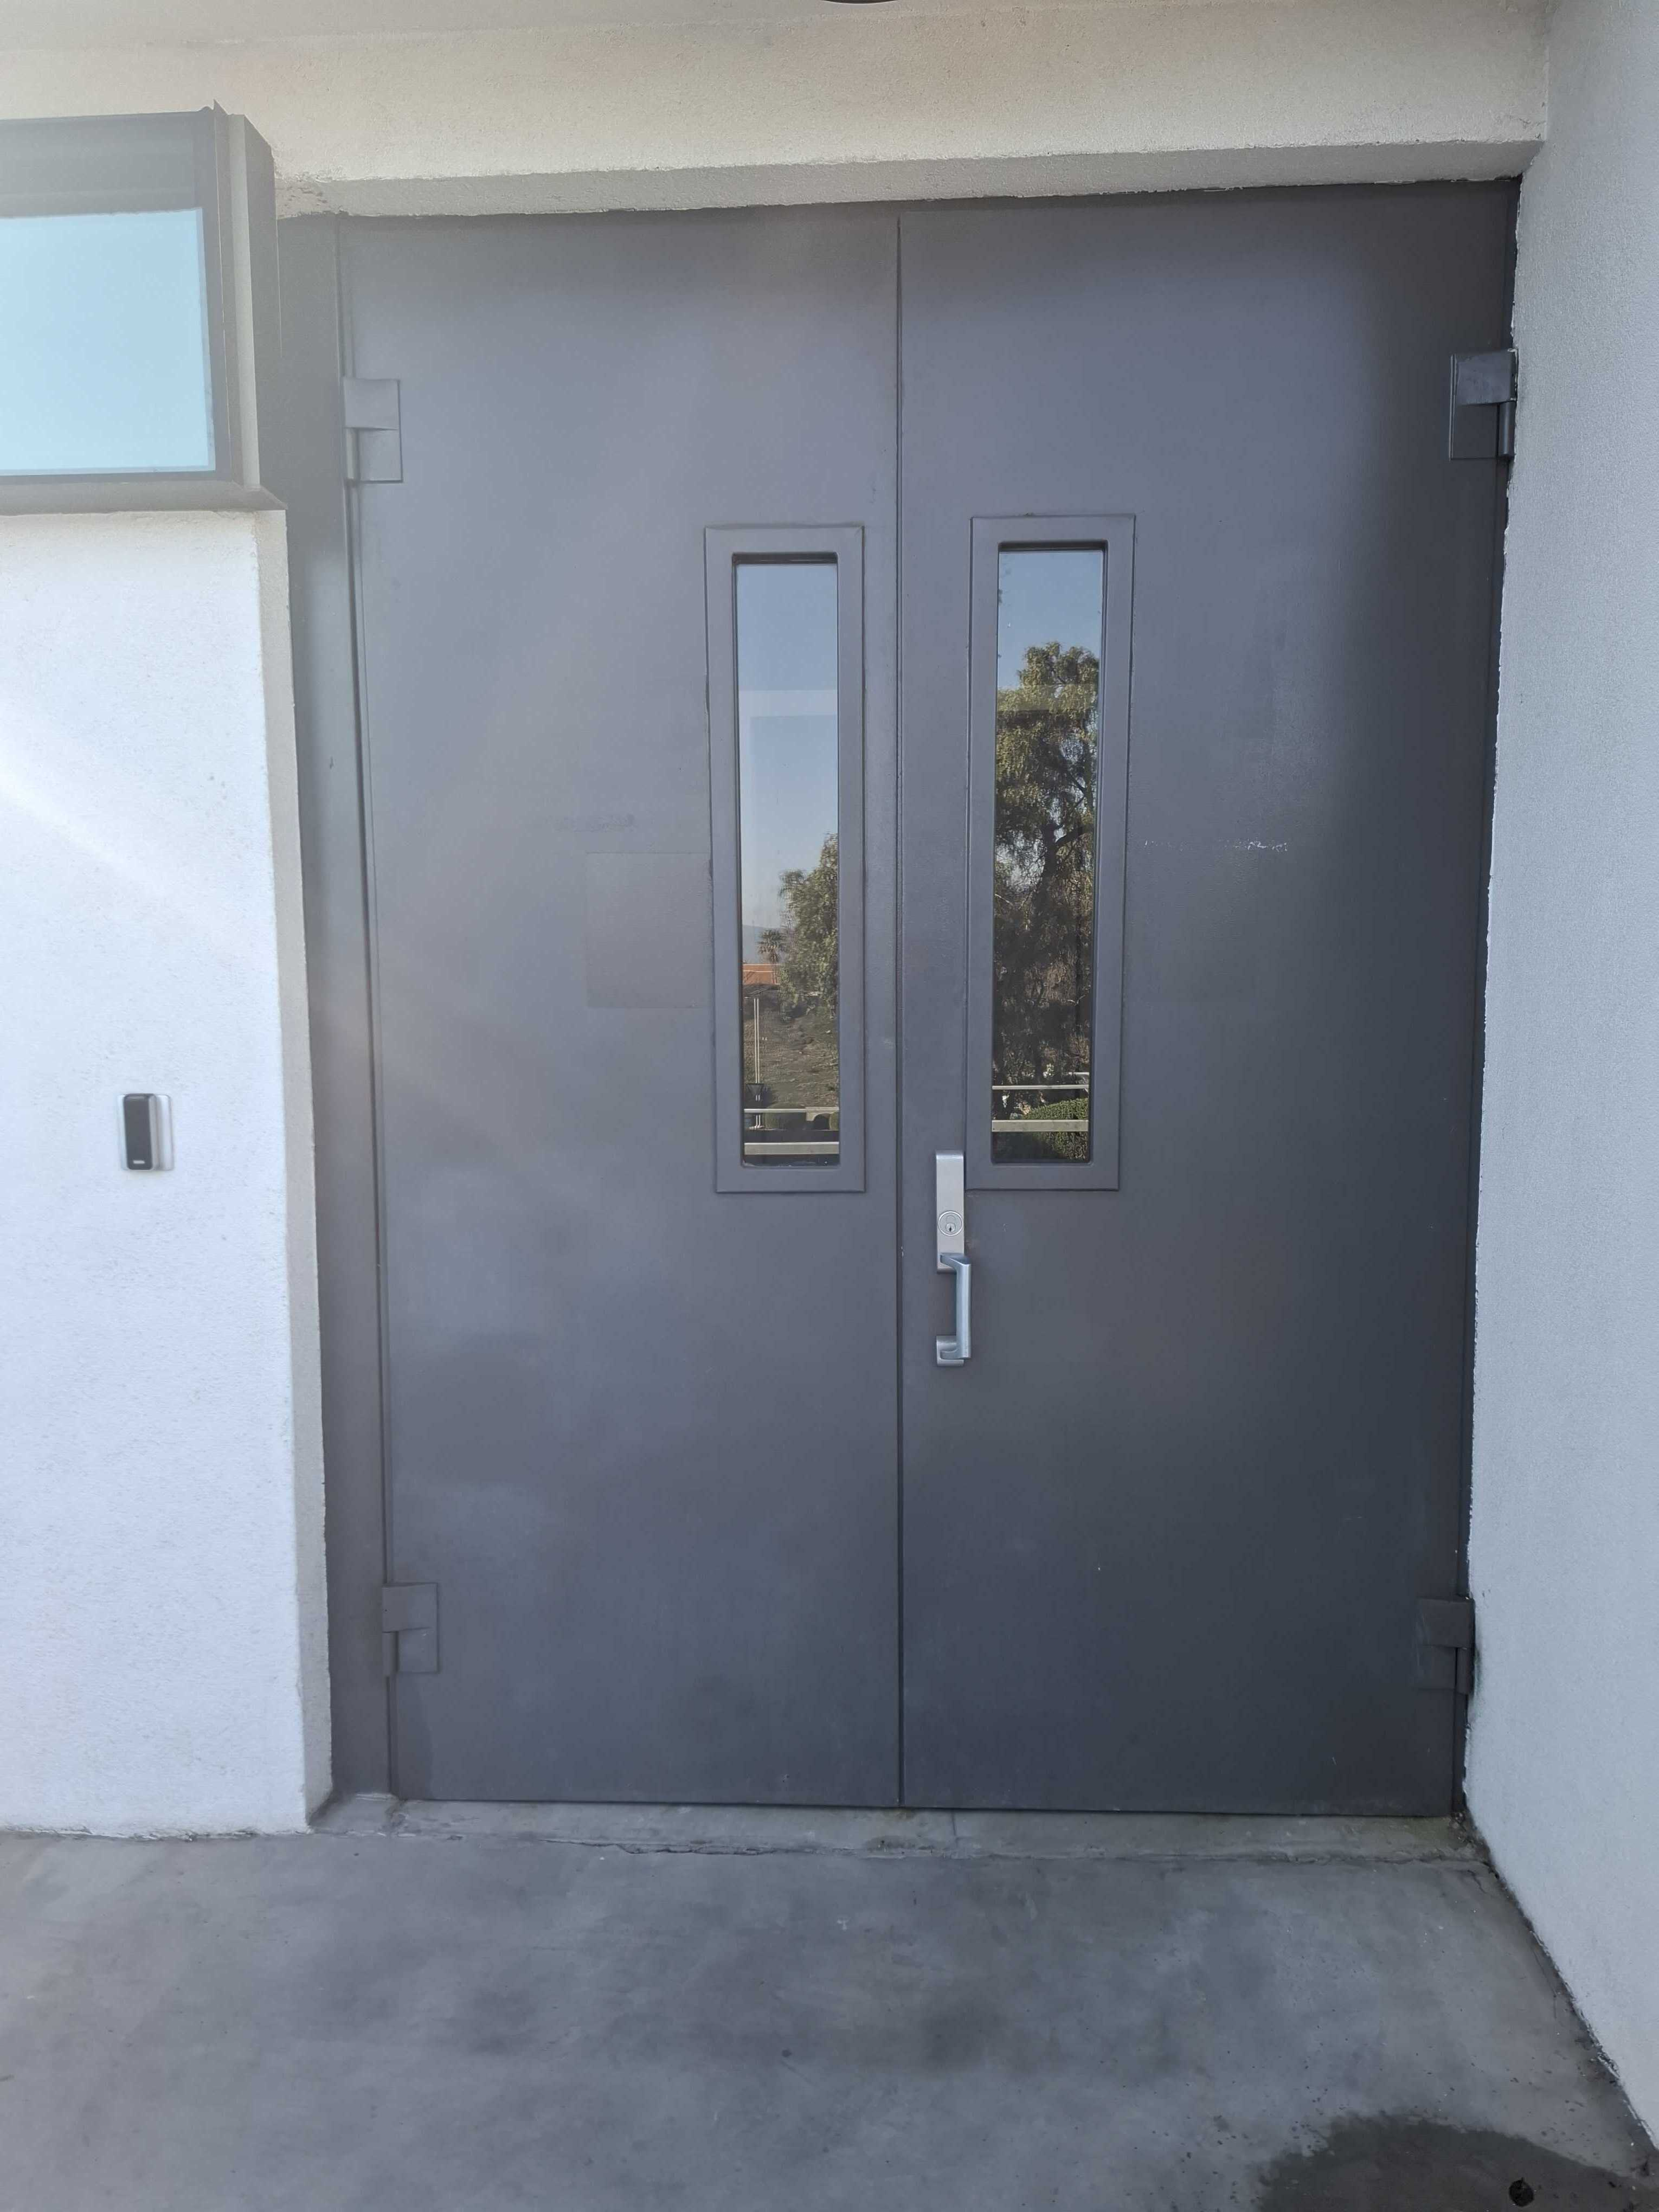
\includegraphics[width=10cm]{15.jpg}
    \centering
    \caption*{Main Gate 1}
  \end{figure}

  \newpage

\begin{figure}
    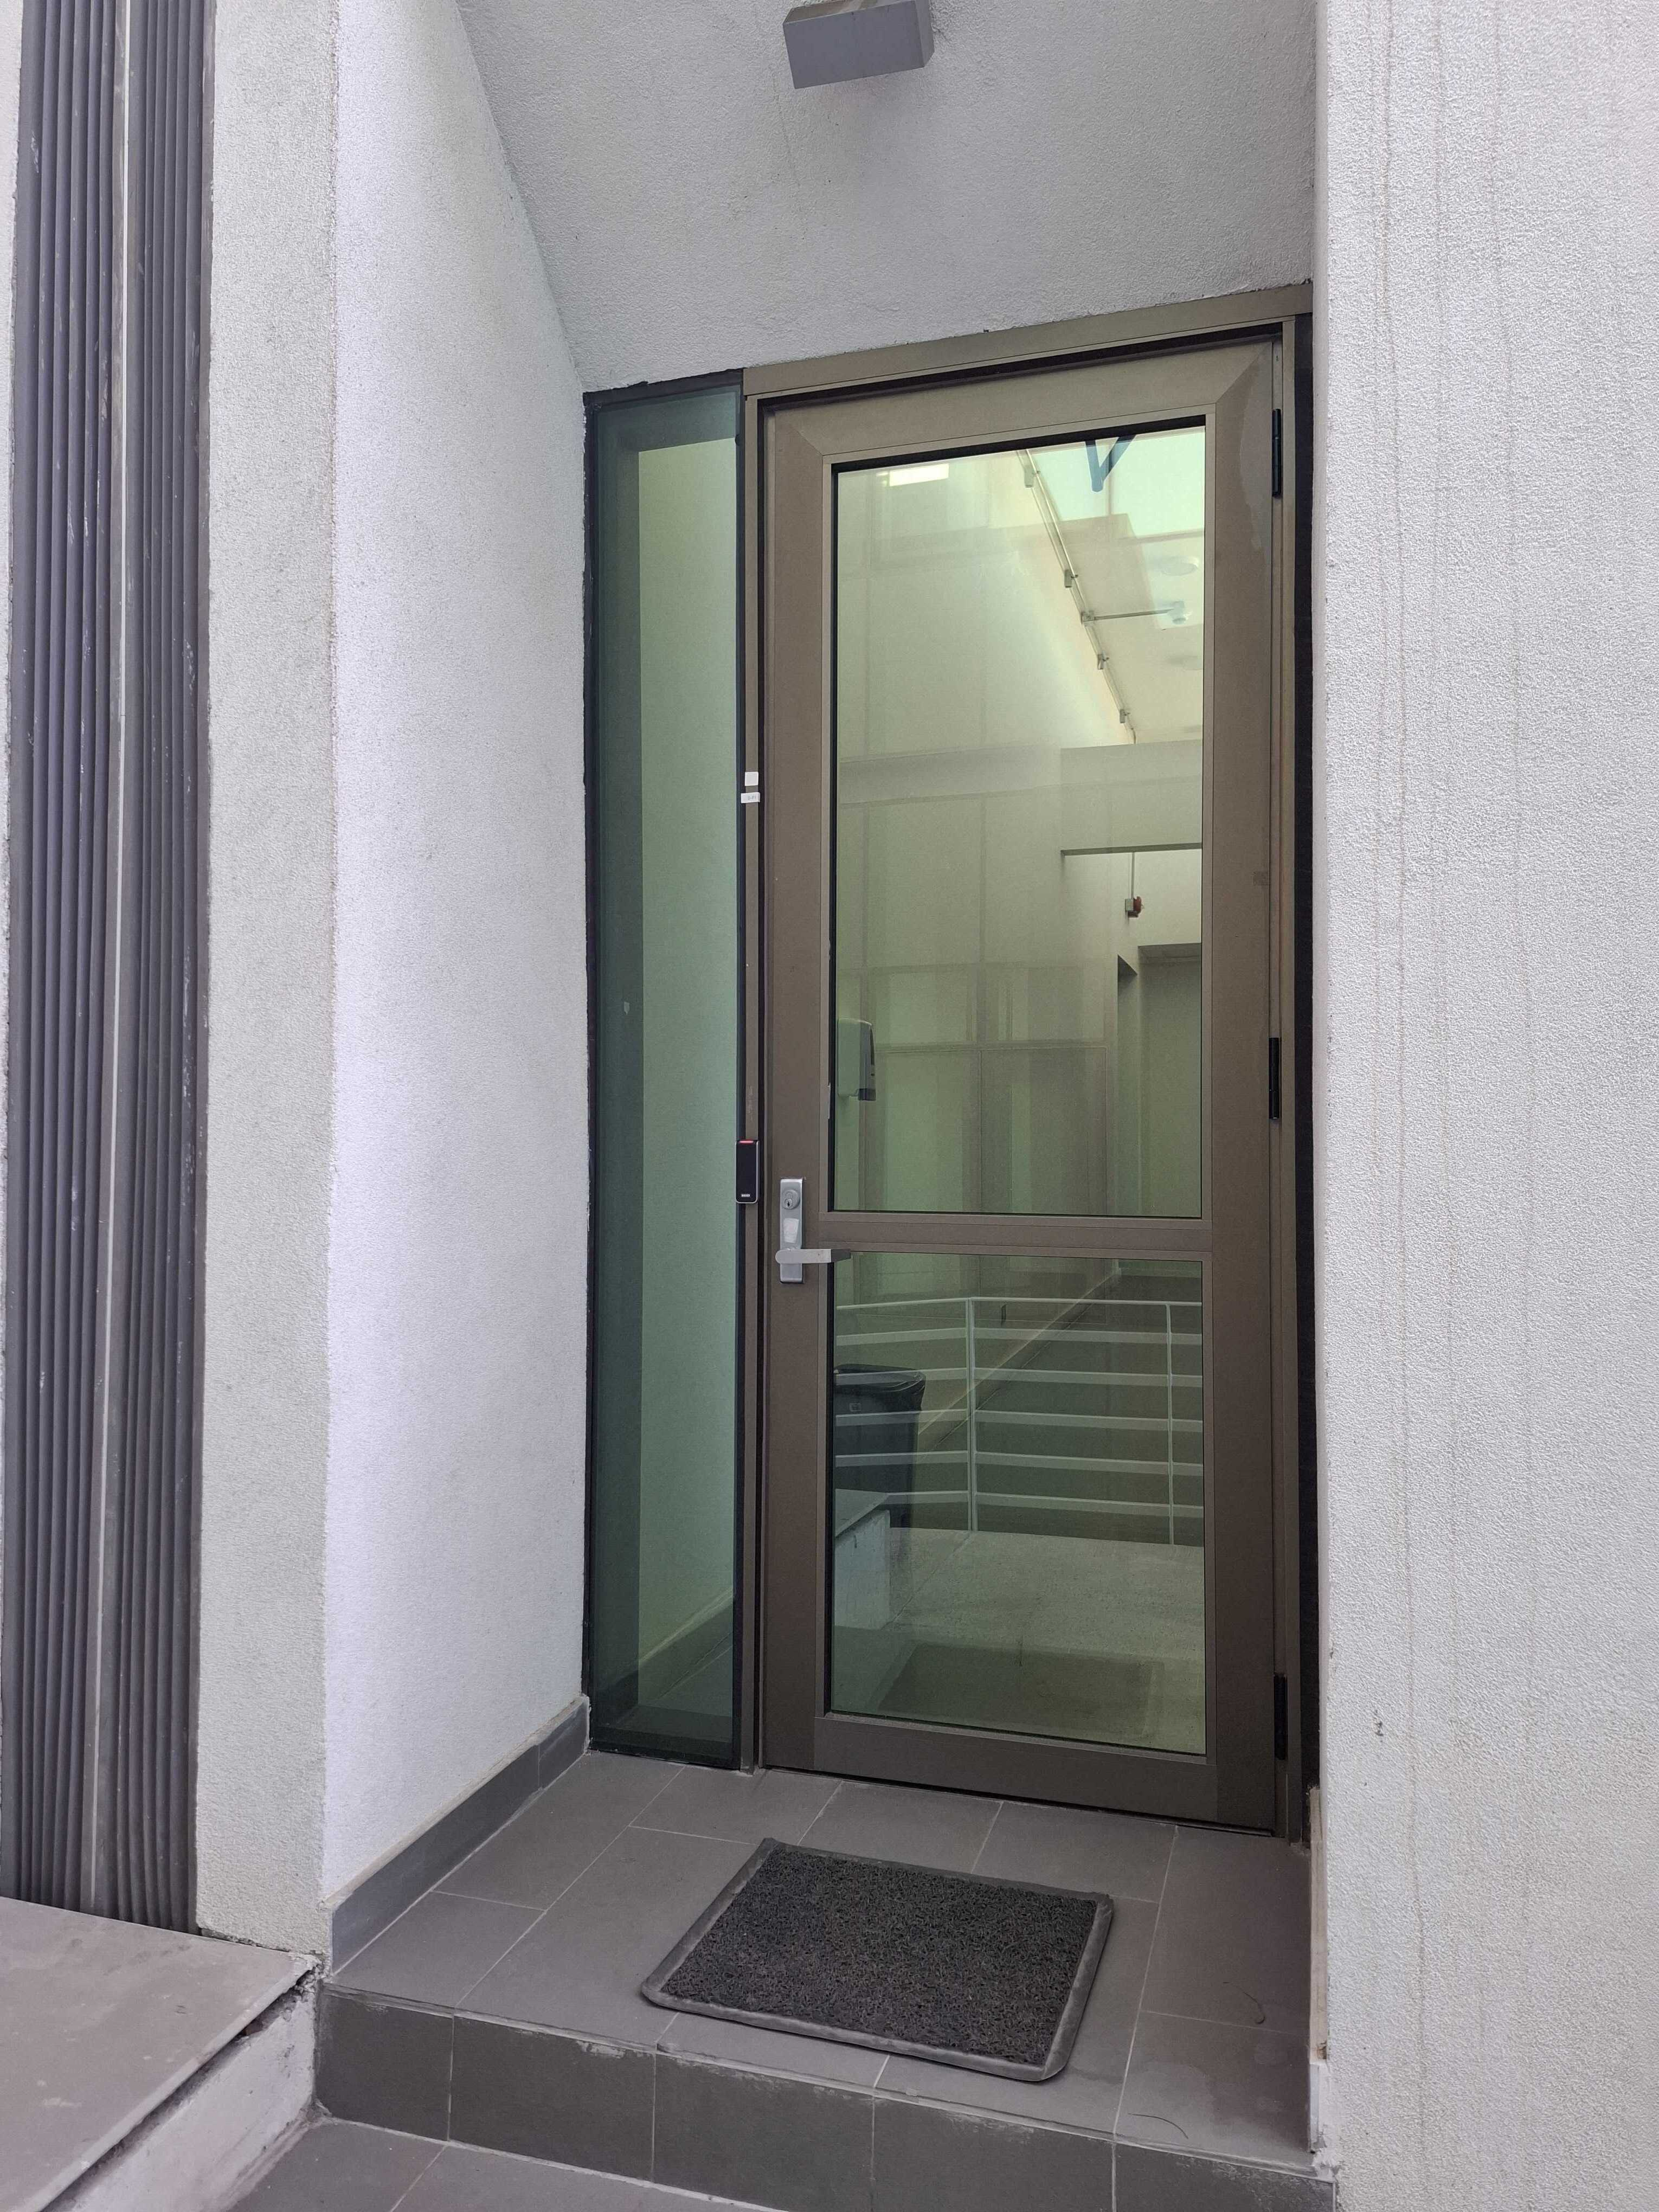
\includegraphics[width=10cm]{16.jpg}
    \centering
    \caption*{Main Gate 2}
  \end{figure}

  \newpage

  \begin{figure}
    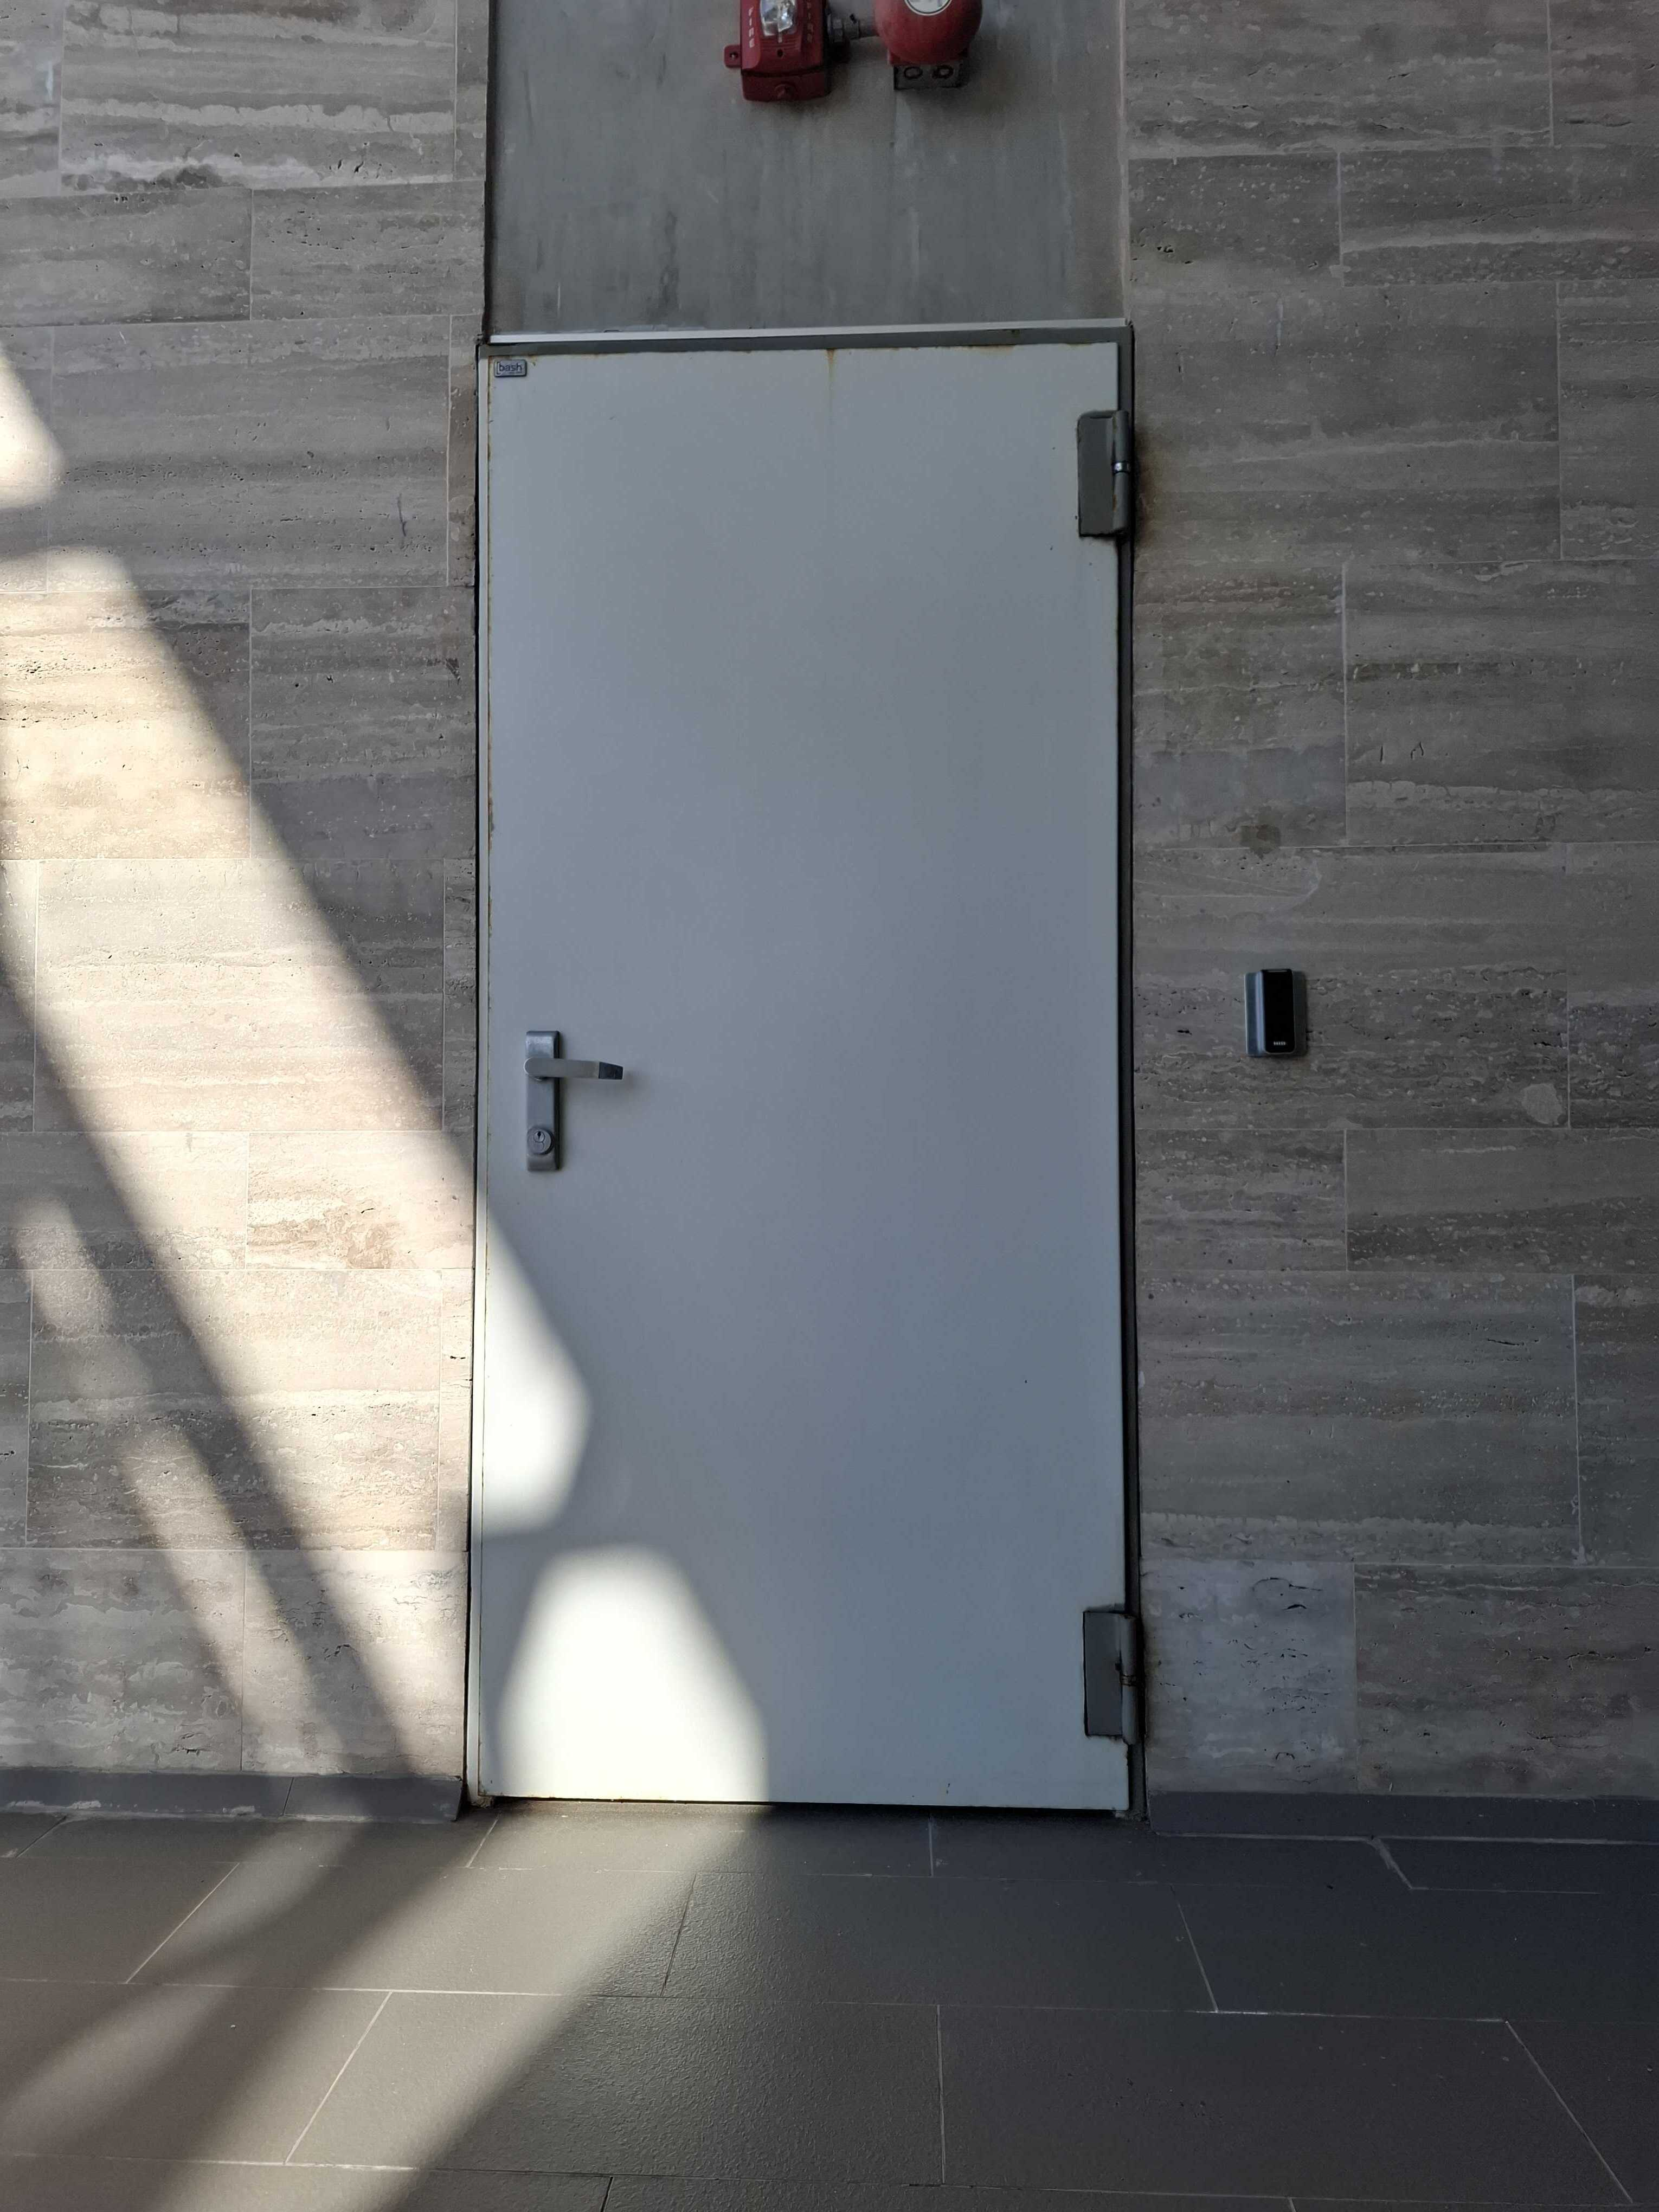
\includegraphics[width=10cm]{17.jpg}
    \centering
    \caption*{Emergency Gate}
  \end{figure}

  \newpage

Also inside the building we have another door to enter the datacenter.

\begin{figure}
    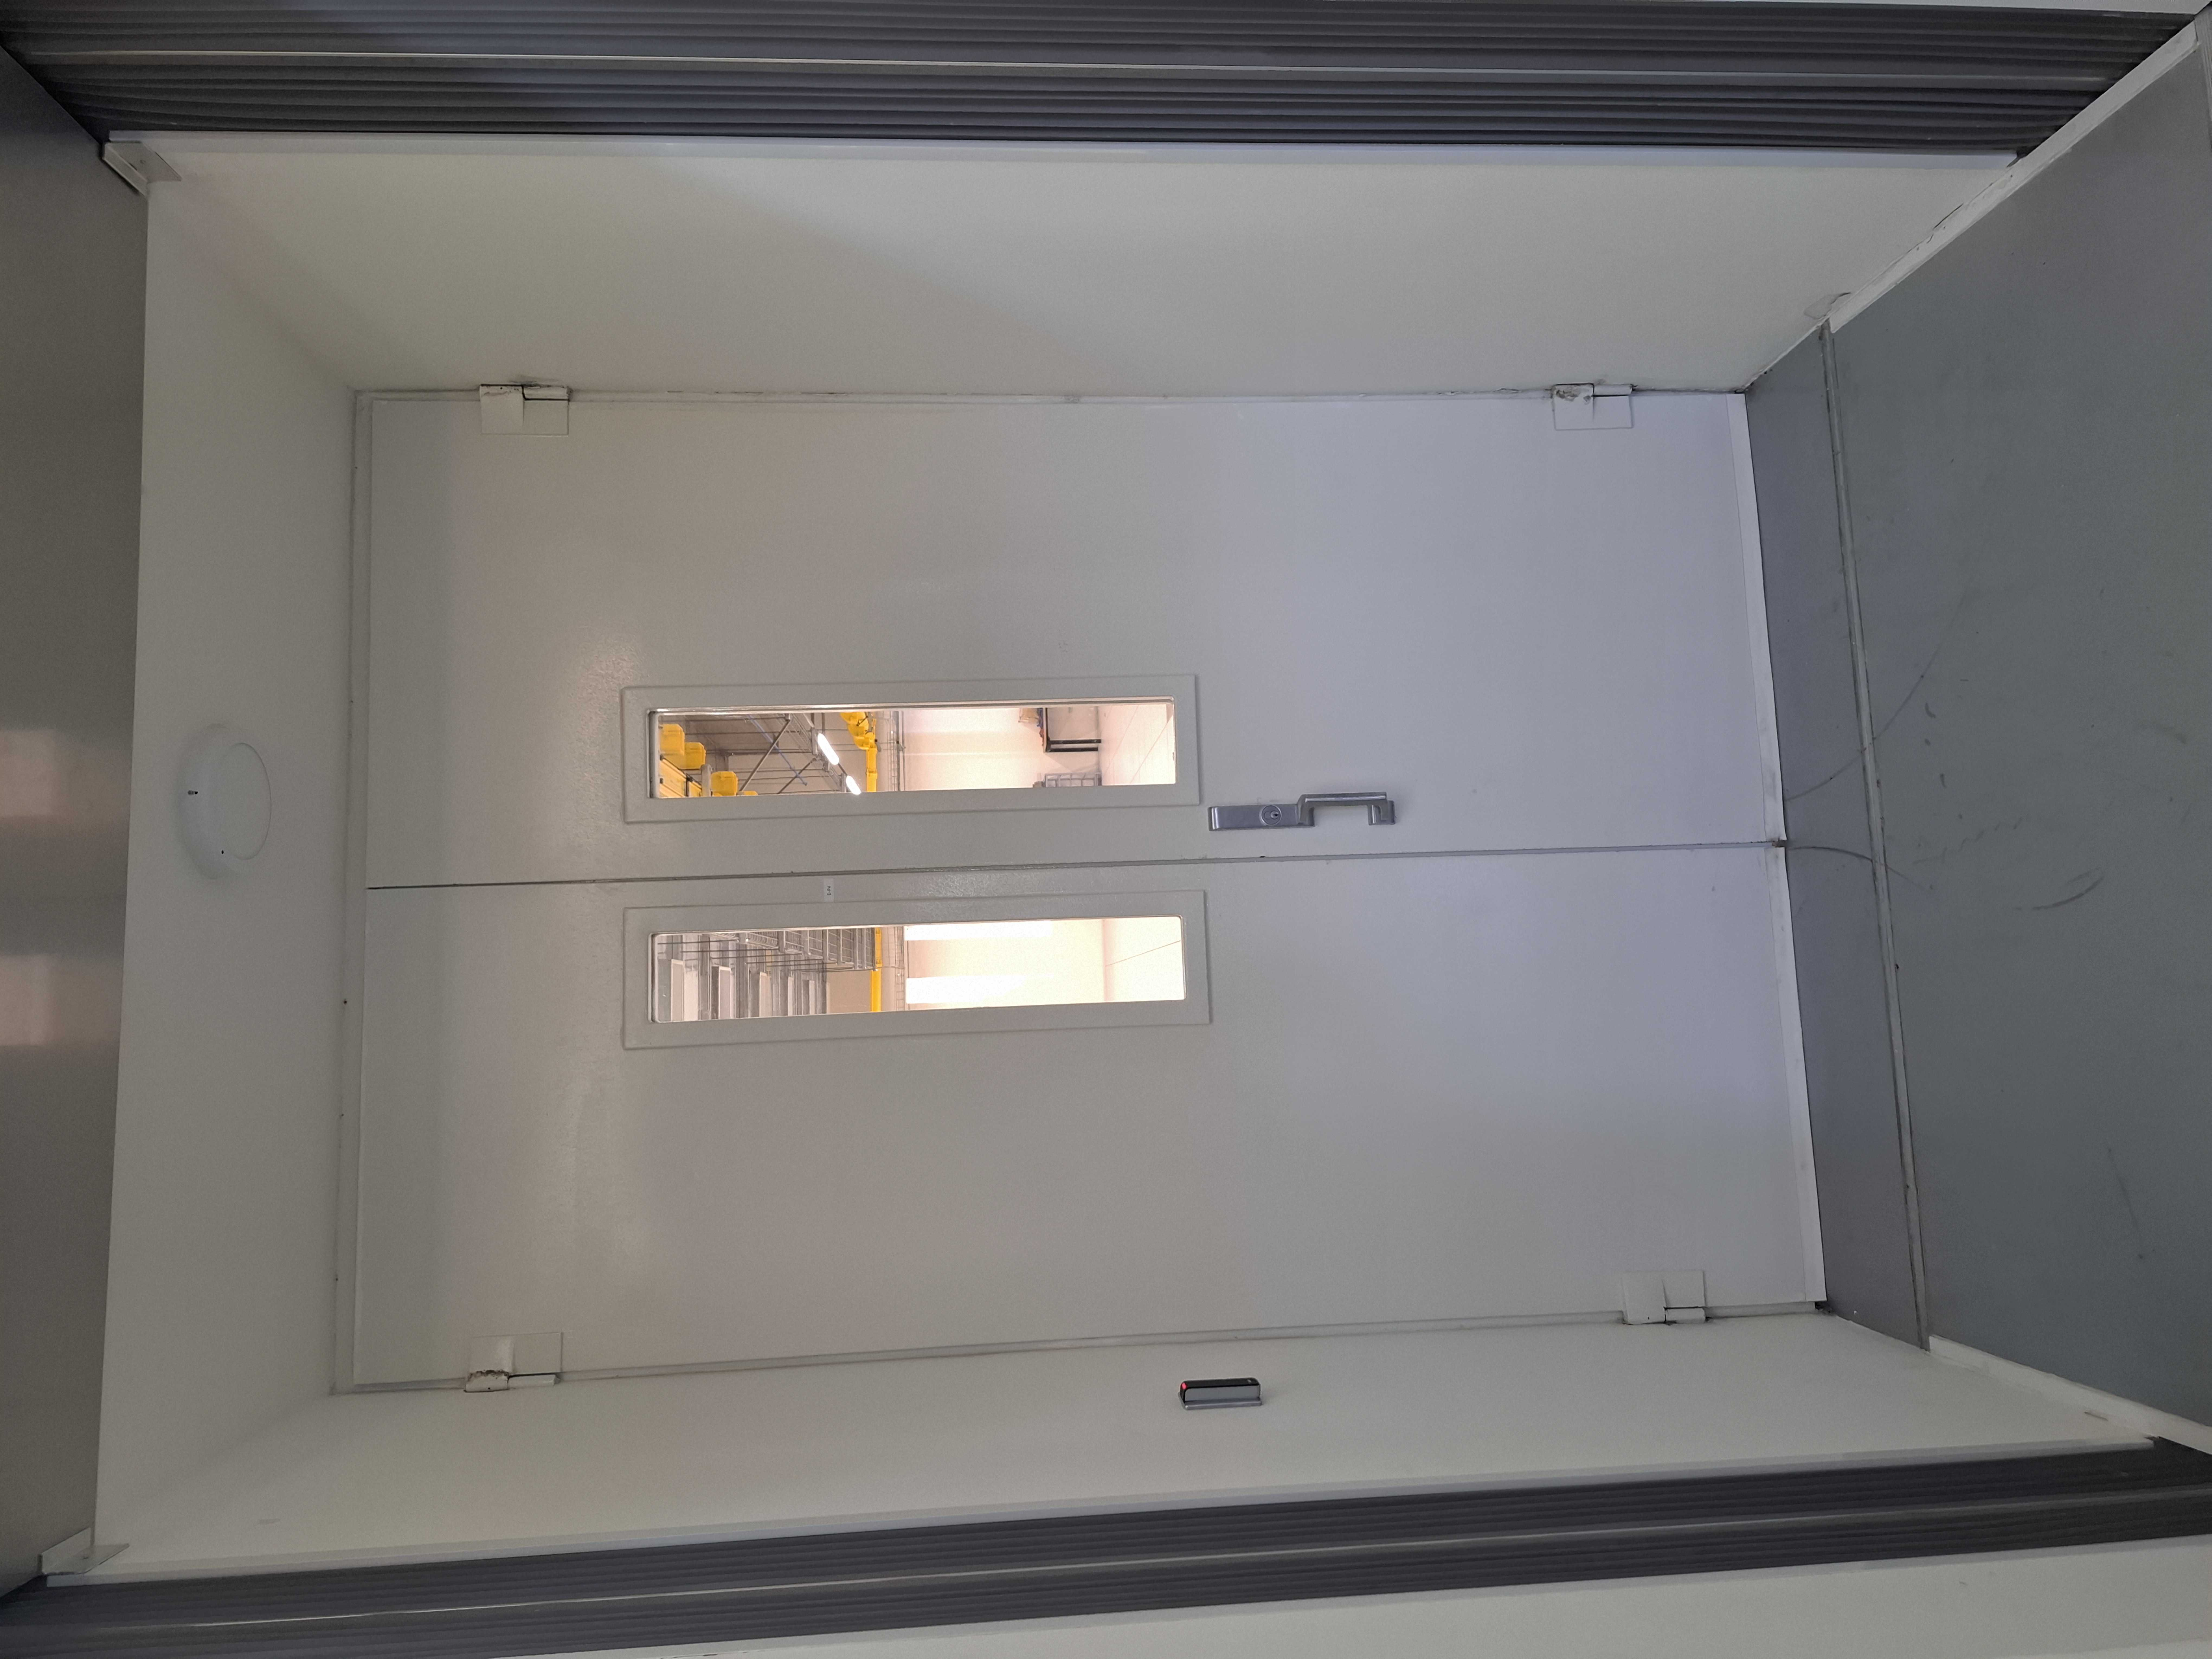
\includegraphics[width=10cm]{18.jpg}
    \centering
    \caption*{Inner Gate}
  \end{figure}

  \newpage

These accesses have their card reader sensors.

\begin{figure}
    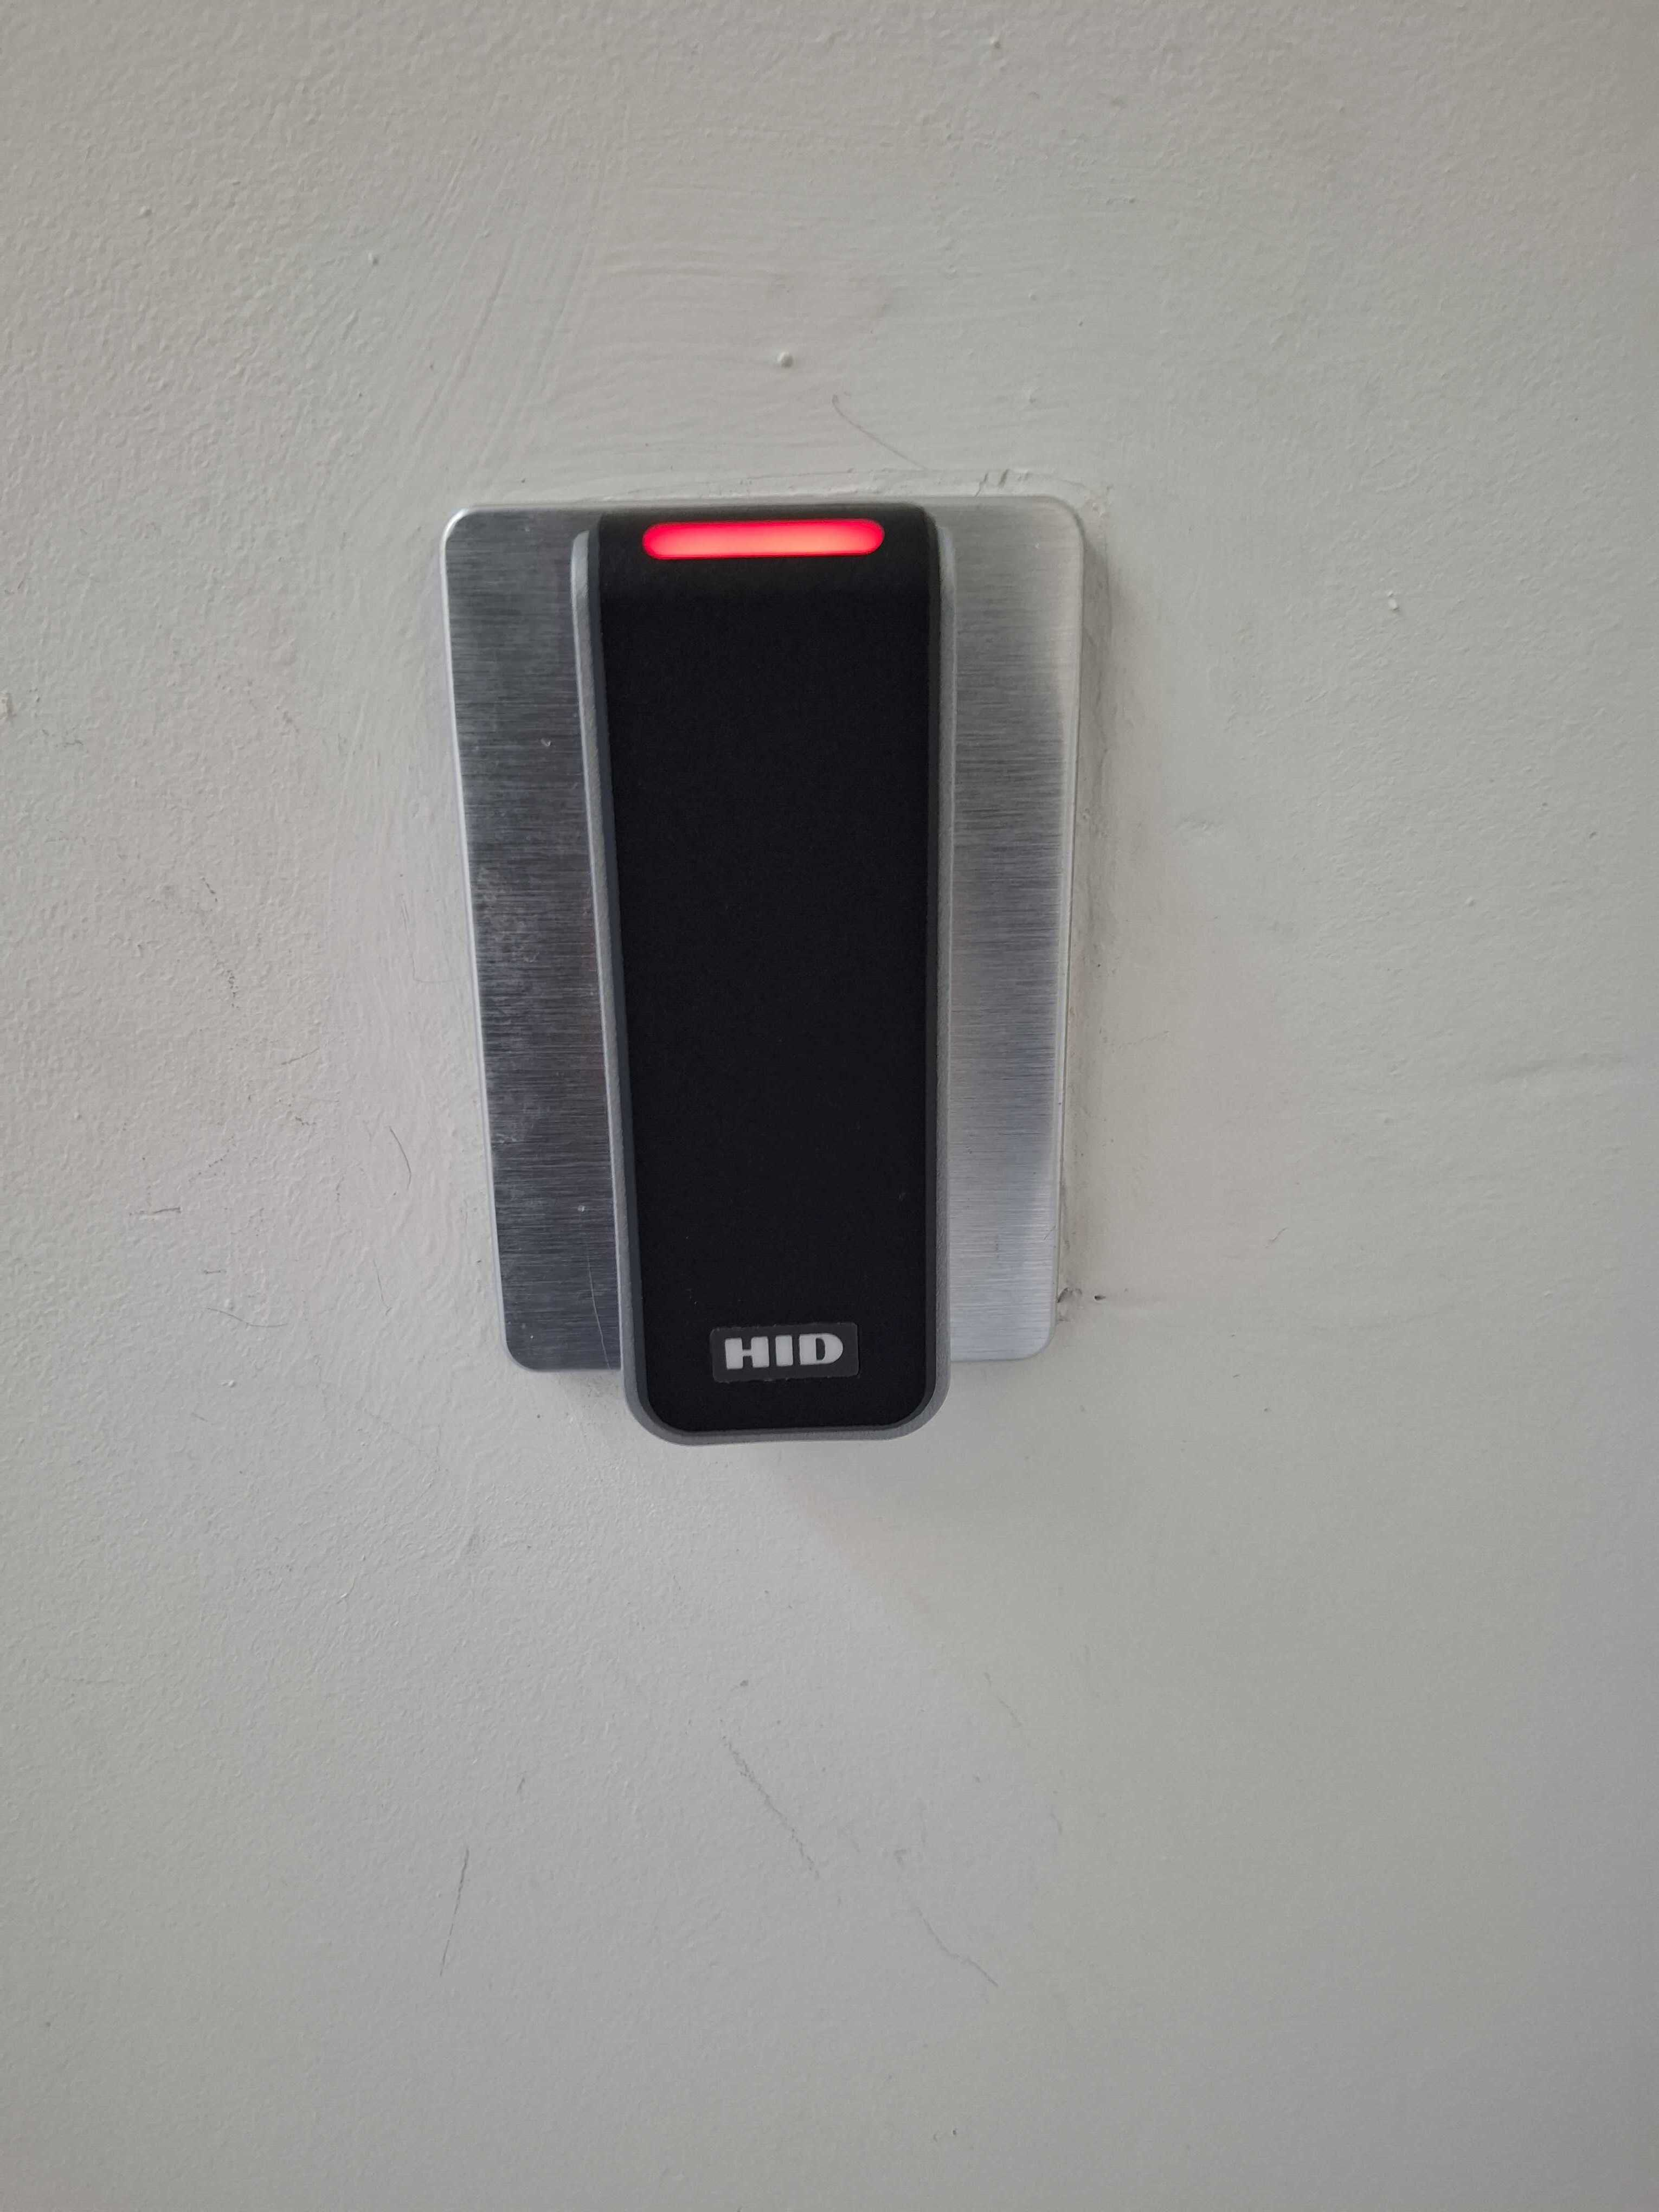
\includegraphics[width=12cm]{19.jpg}
    \centering
    \caption*{Door Sensor}
  \end{figure}

The accesses must be provided by Noirlab.

\section{Access Control Main Gate, Cerro Pachón}

This site does not yet have card access control, but we are in the process of acquiring the same system that is working at the aura site in La Serena.

\begin{figure}
    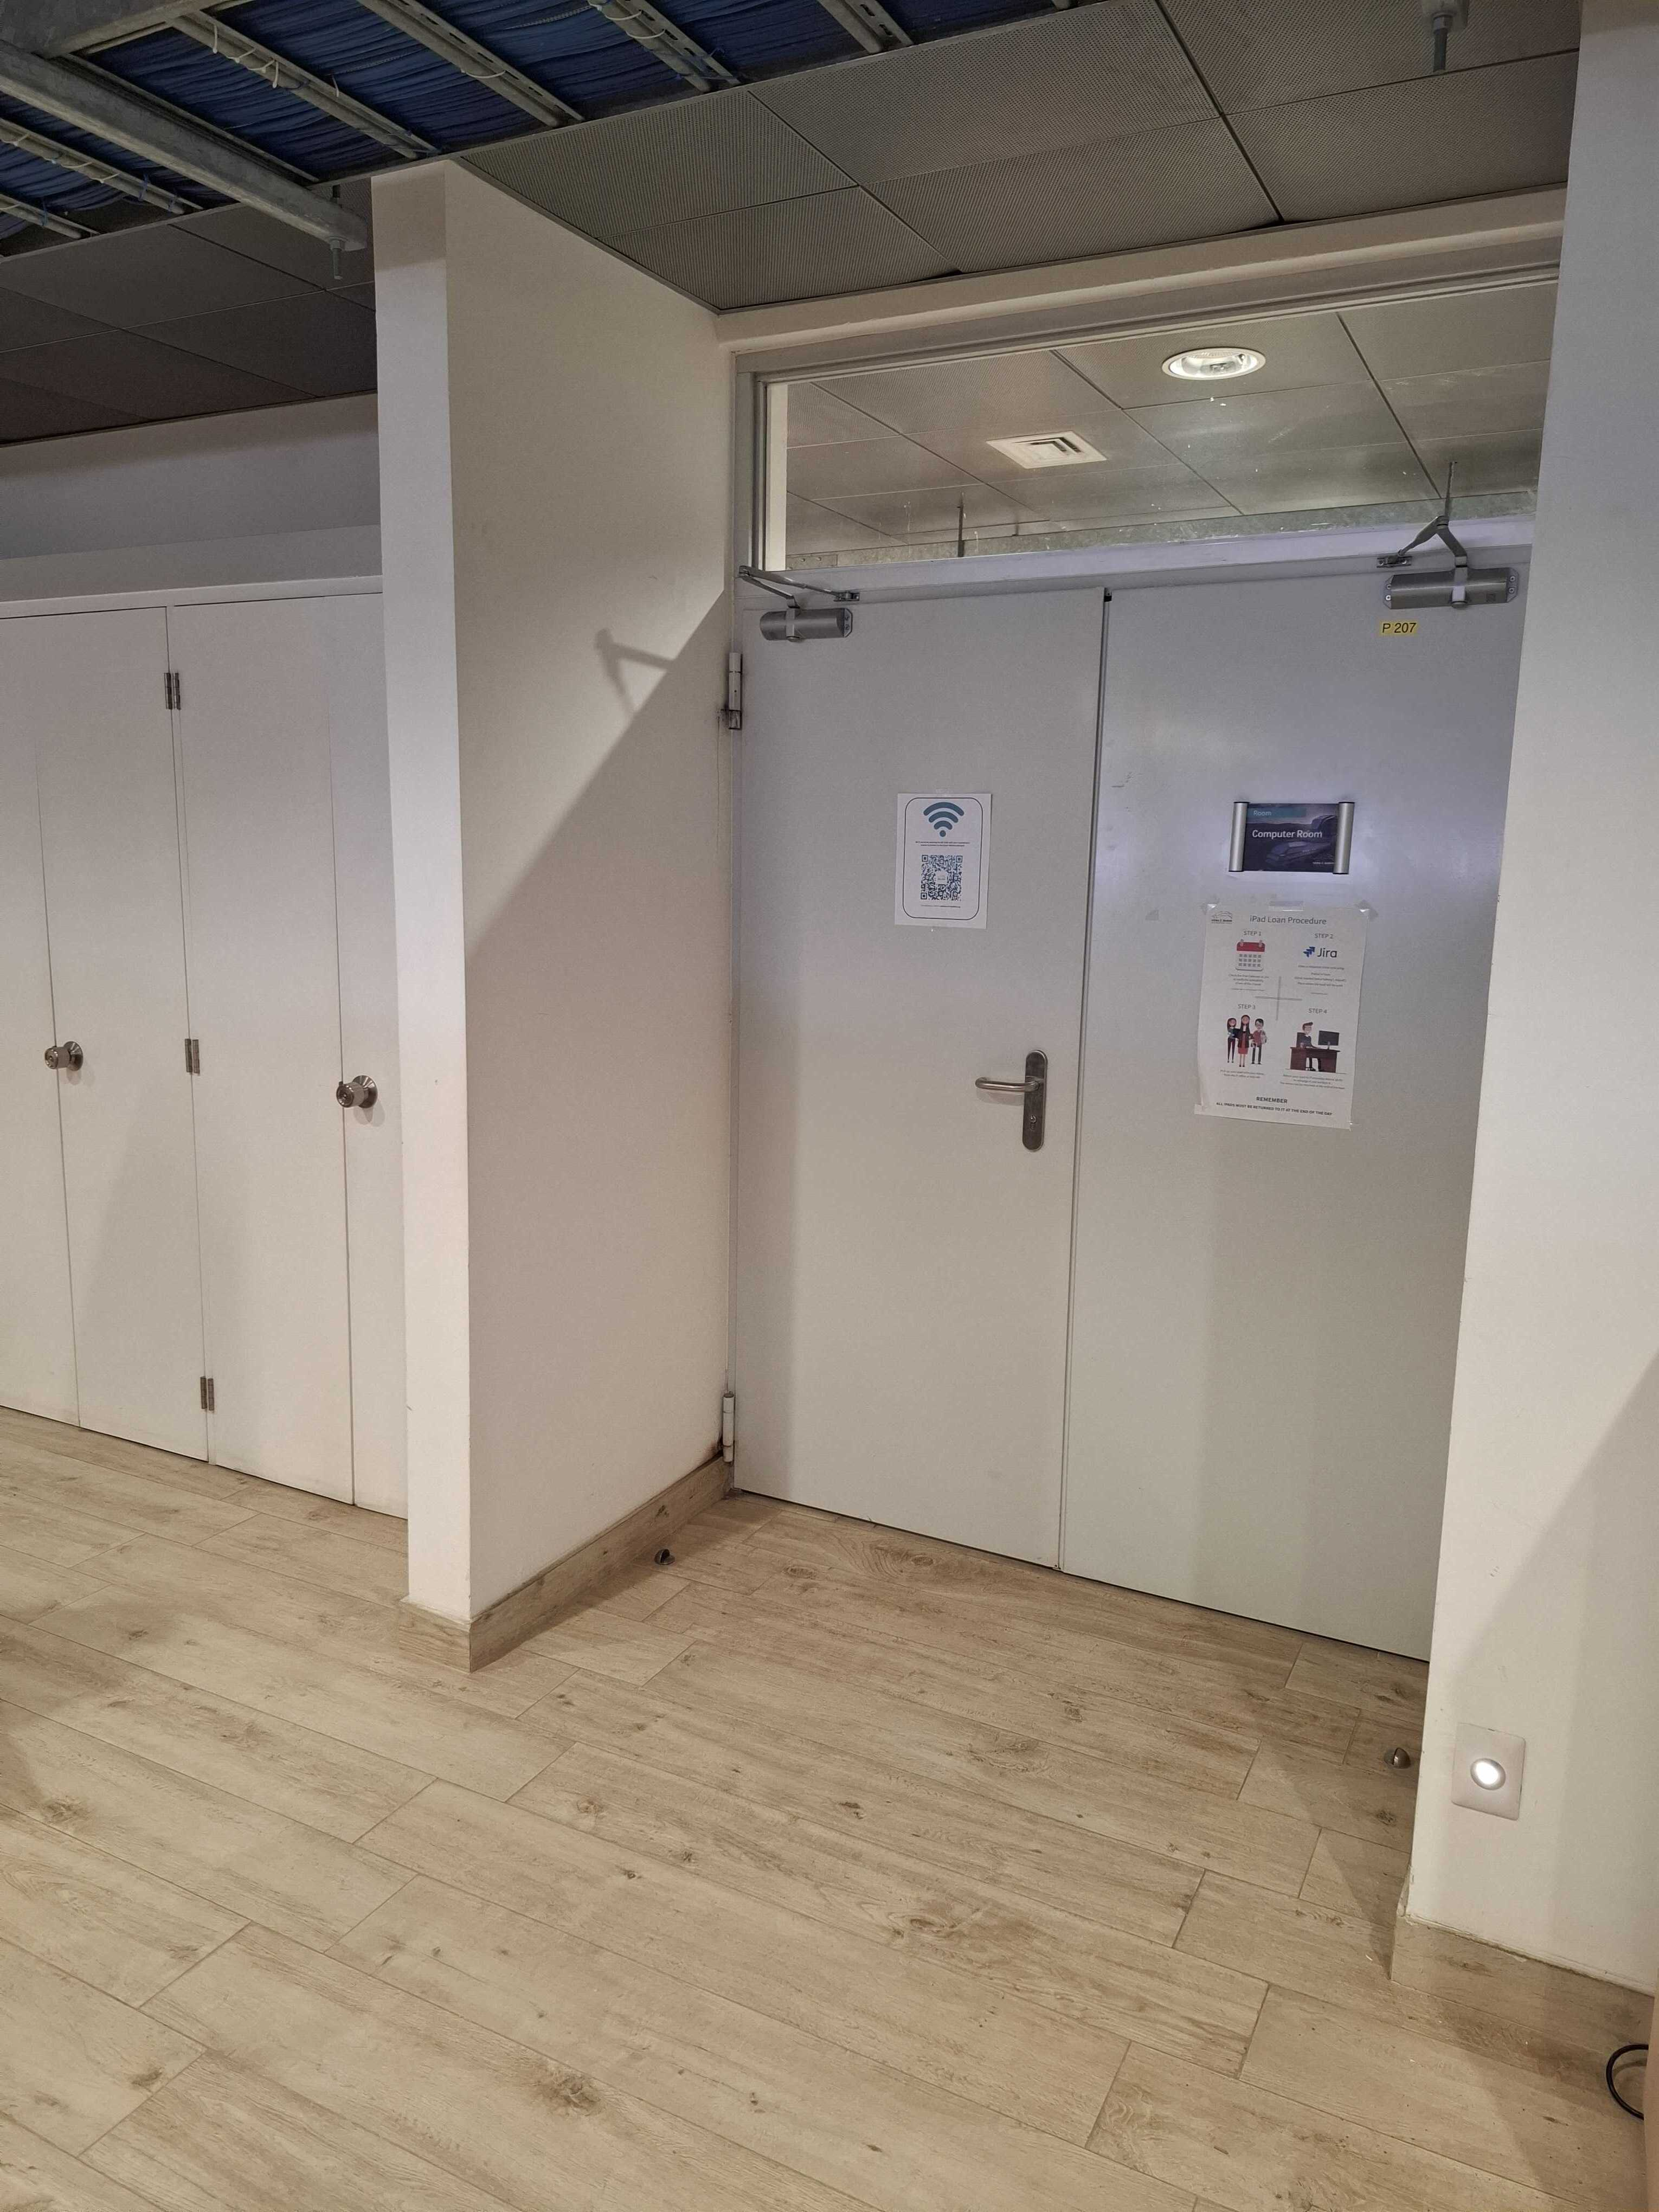
\includegraphics[width=7cm]{20.jpg}
    \centering
    \caption*{SDC Outside Gate}
  \end{figure}
  \begin{figure}
    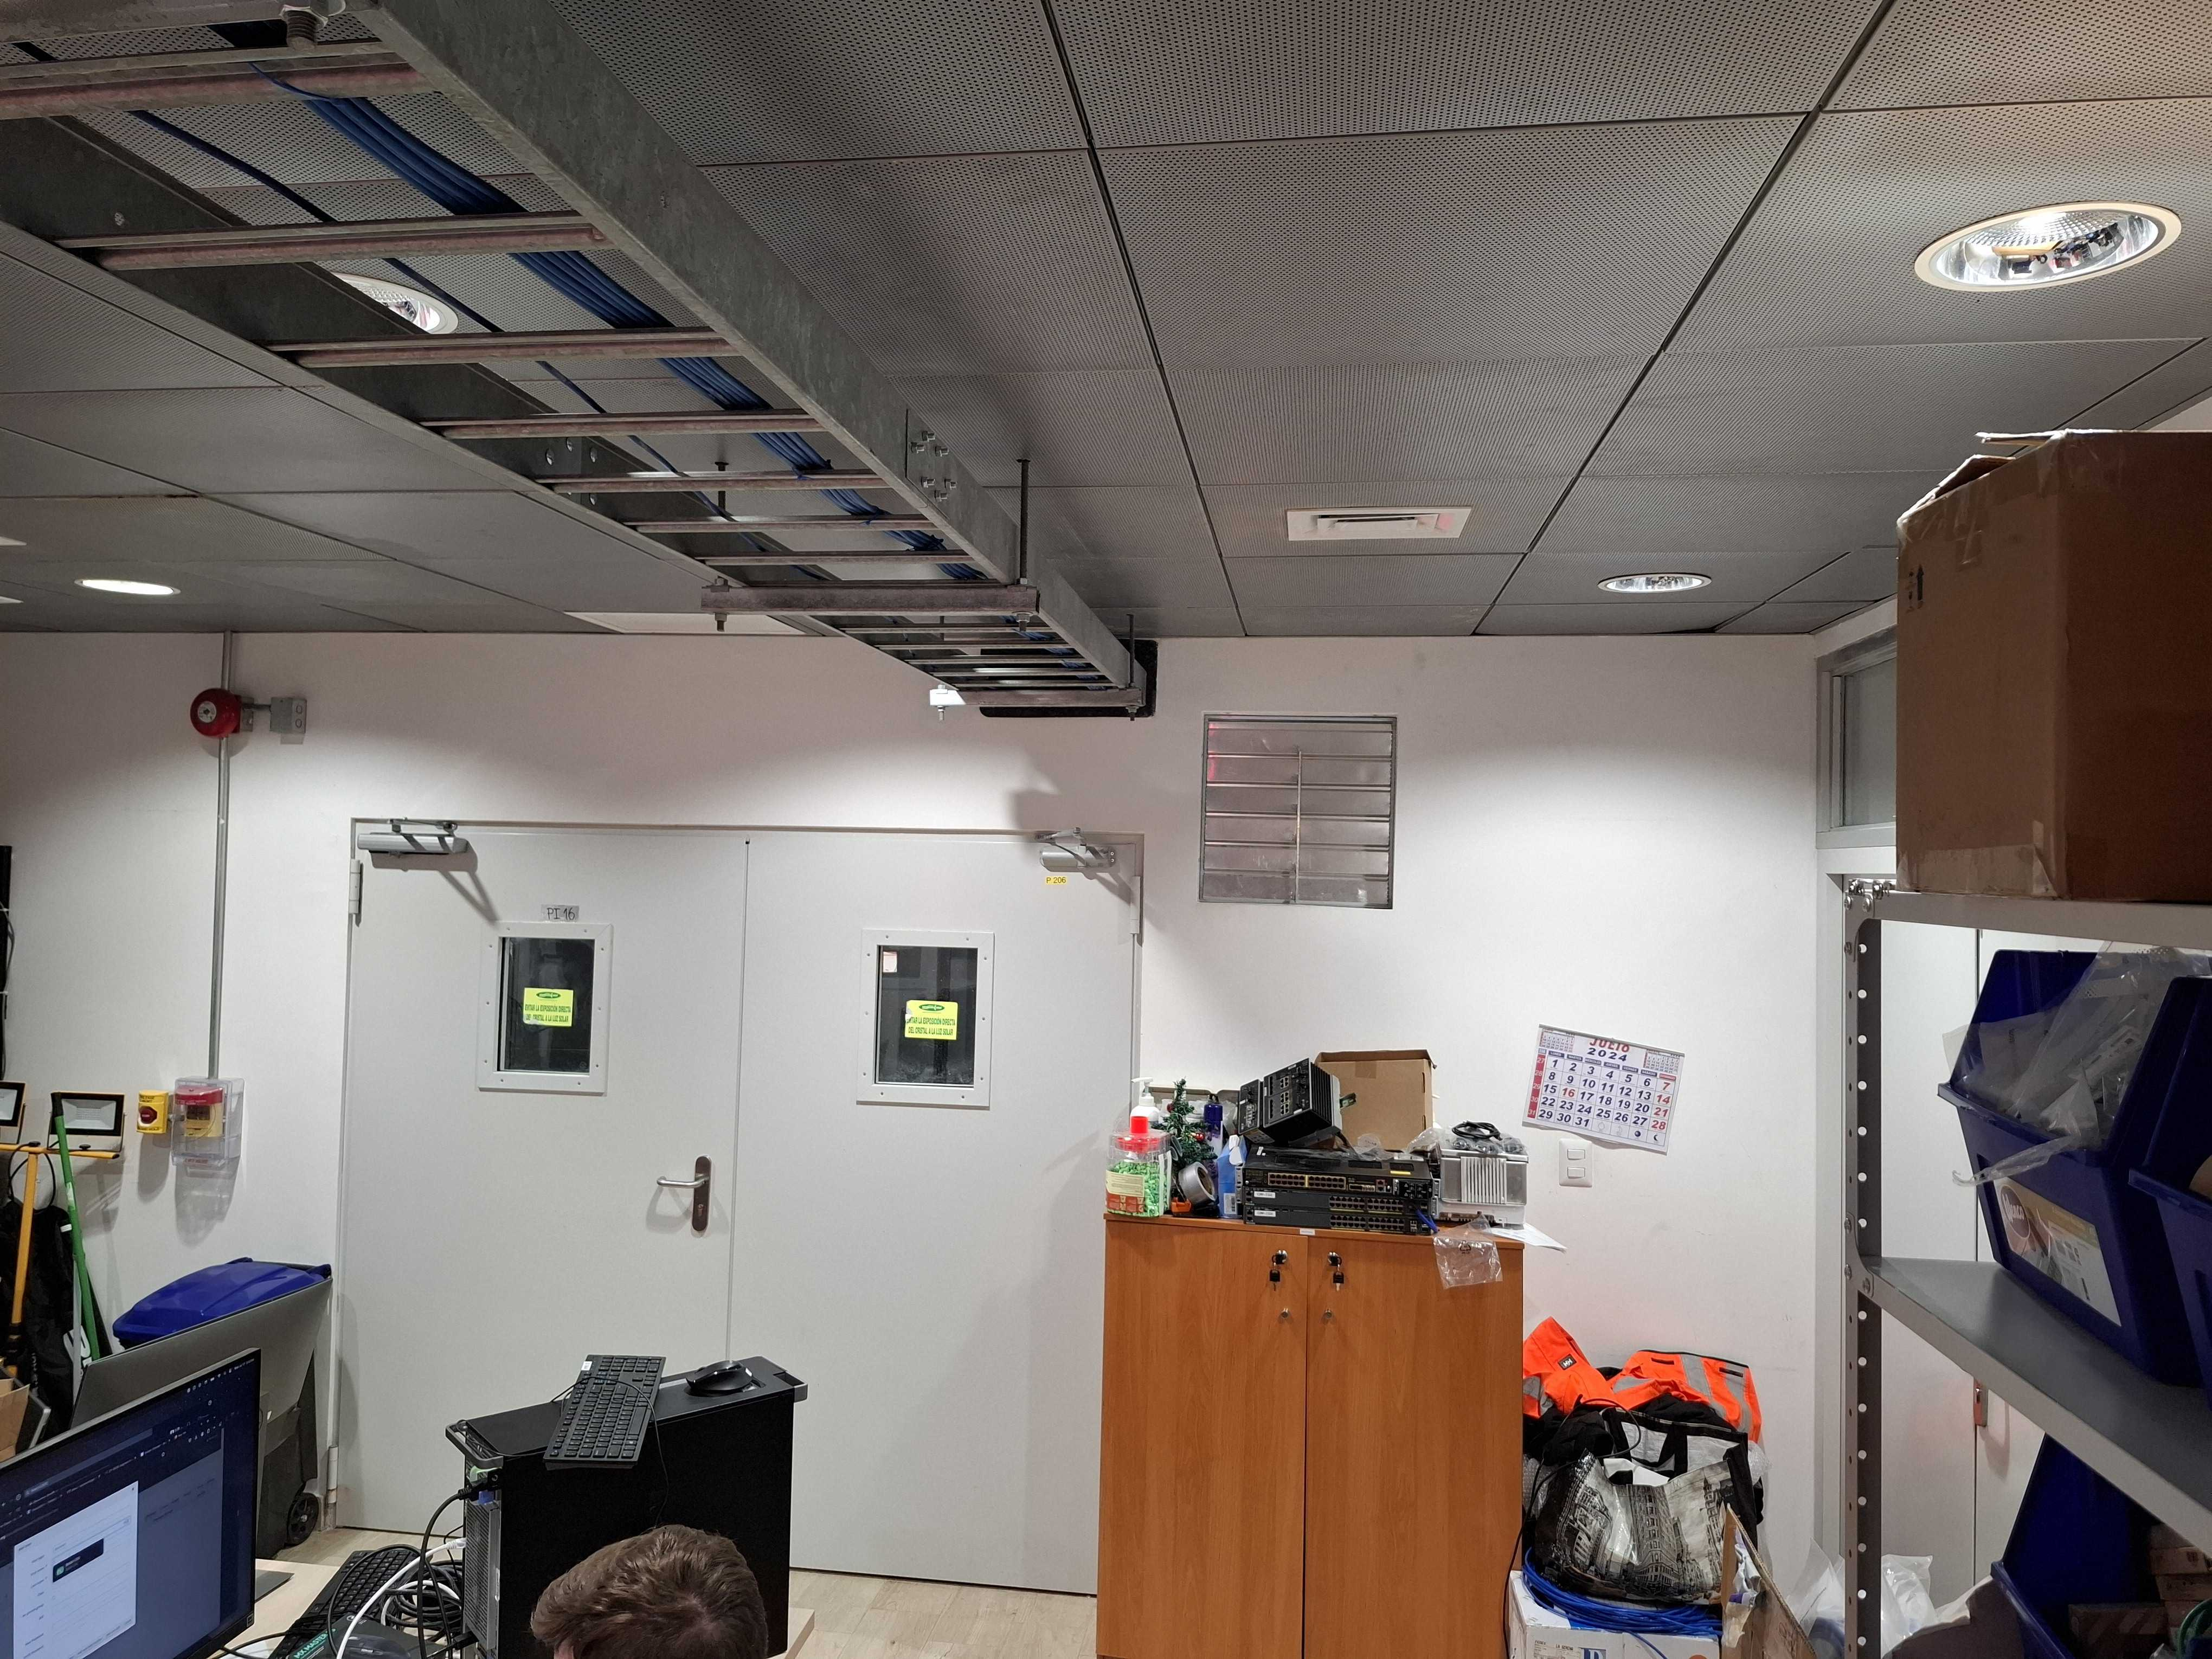
\includegraphics[width=7cm]{21.jpg}
    \centering
    \caption*{SDC Inner Gate}
  \end{figure}

\section{Access and movement control through cameras}

Within the datacenter facilities, cameras were installed to observe the rack corridors, both in the front and back of the racks. The idea of these devices is to be able to monitor the movements inside the datacenter.

To obtain access to these images, authorization is required through IT and also if your business profile requires it.

\subsection{Datacenter La Serena}

Here we have cameras pointing to row B in the front and back of the racks.

\begin{figure}
    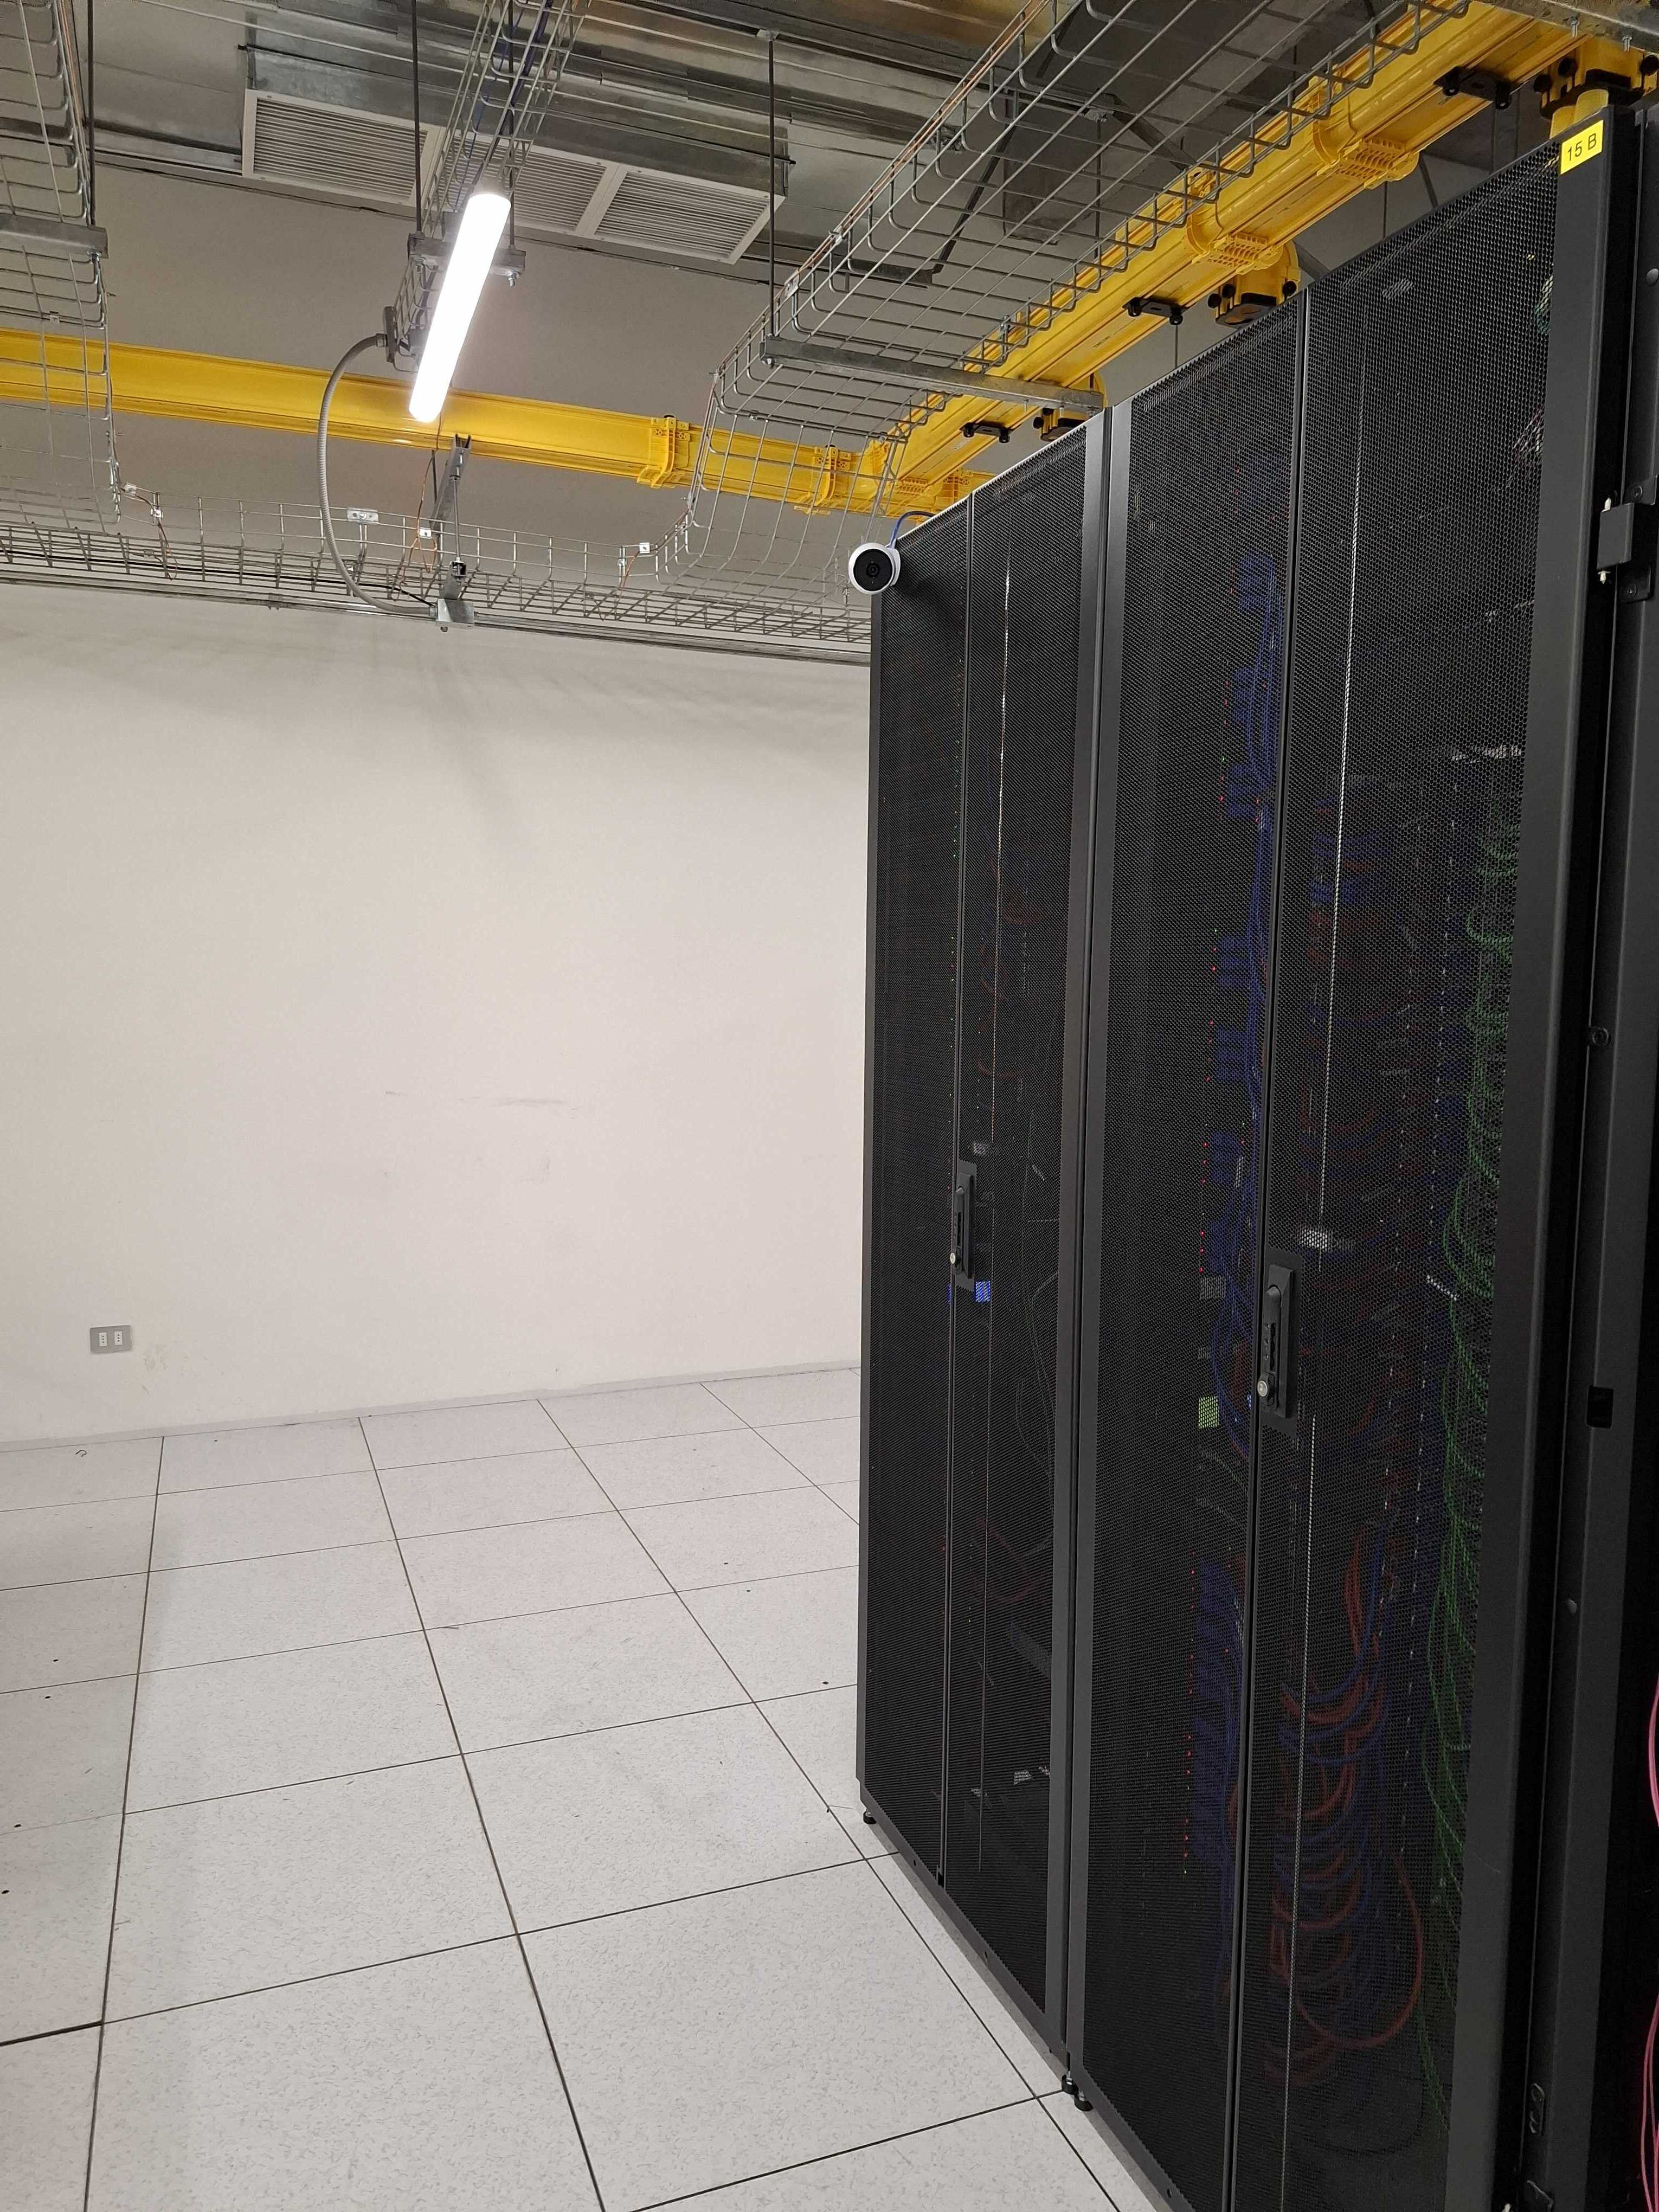
\includegraphics[width=8cm]{7.jpg}
    \centering
    \caption*{Hot Corridor Camera}
  \end{figure}

  \newpage

  \begin{figure}
    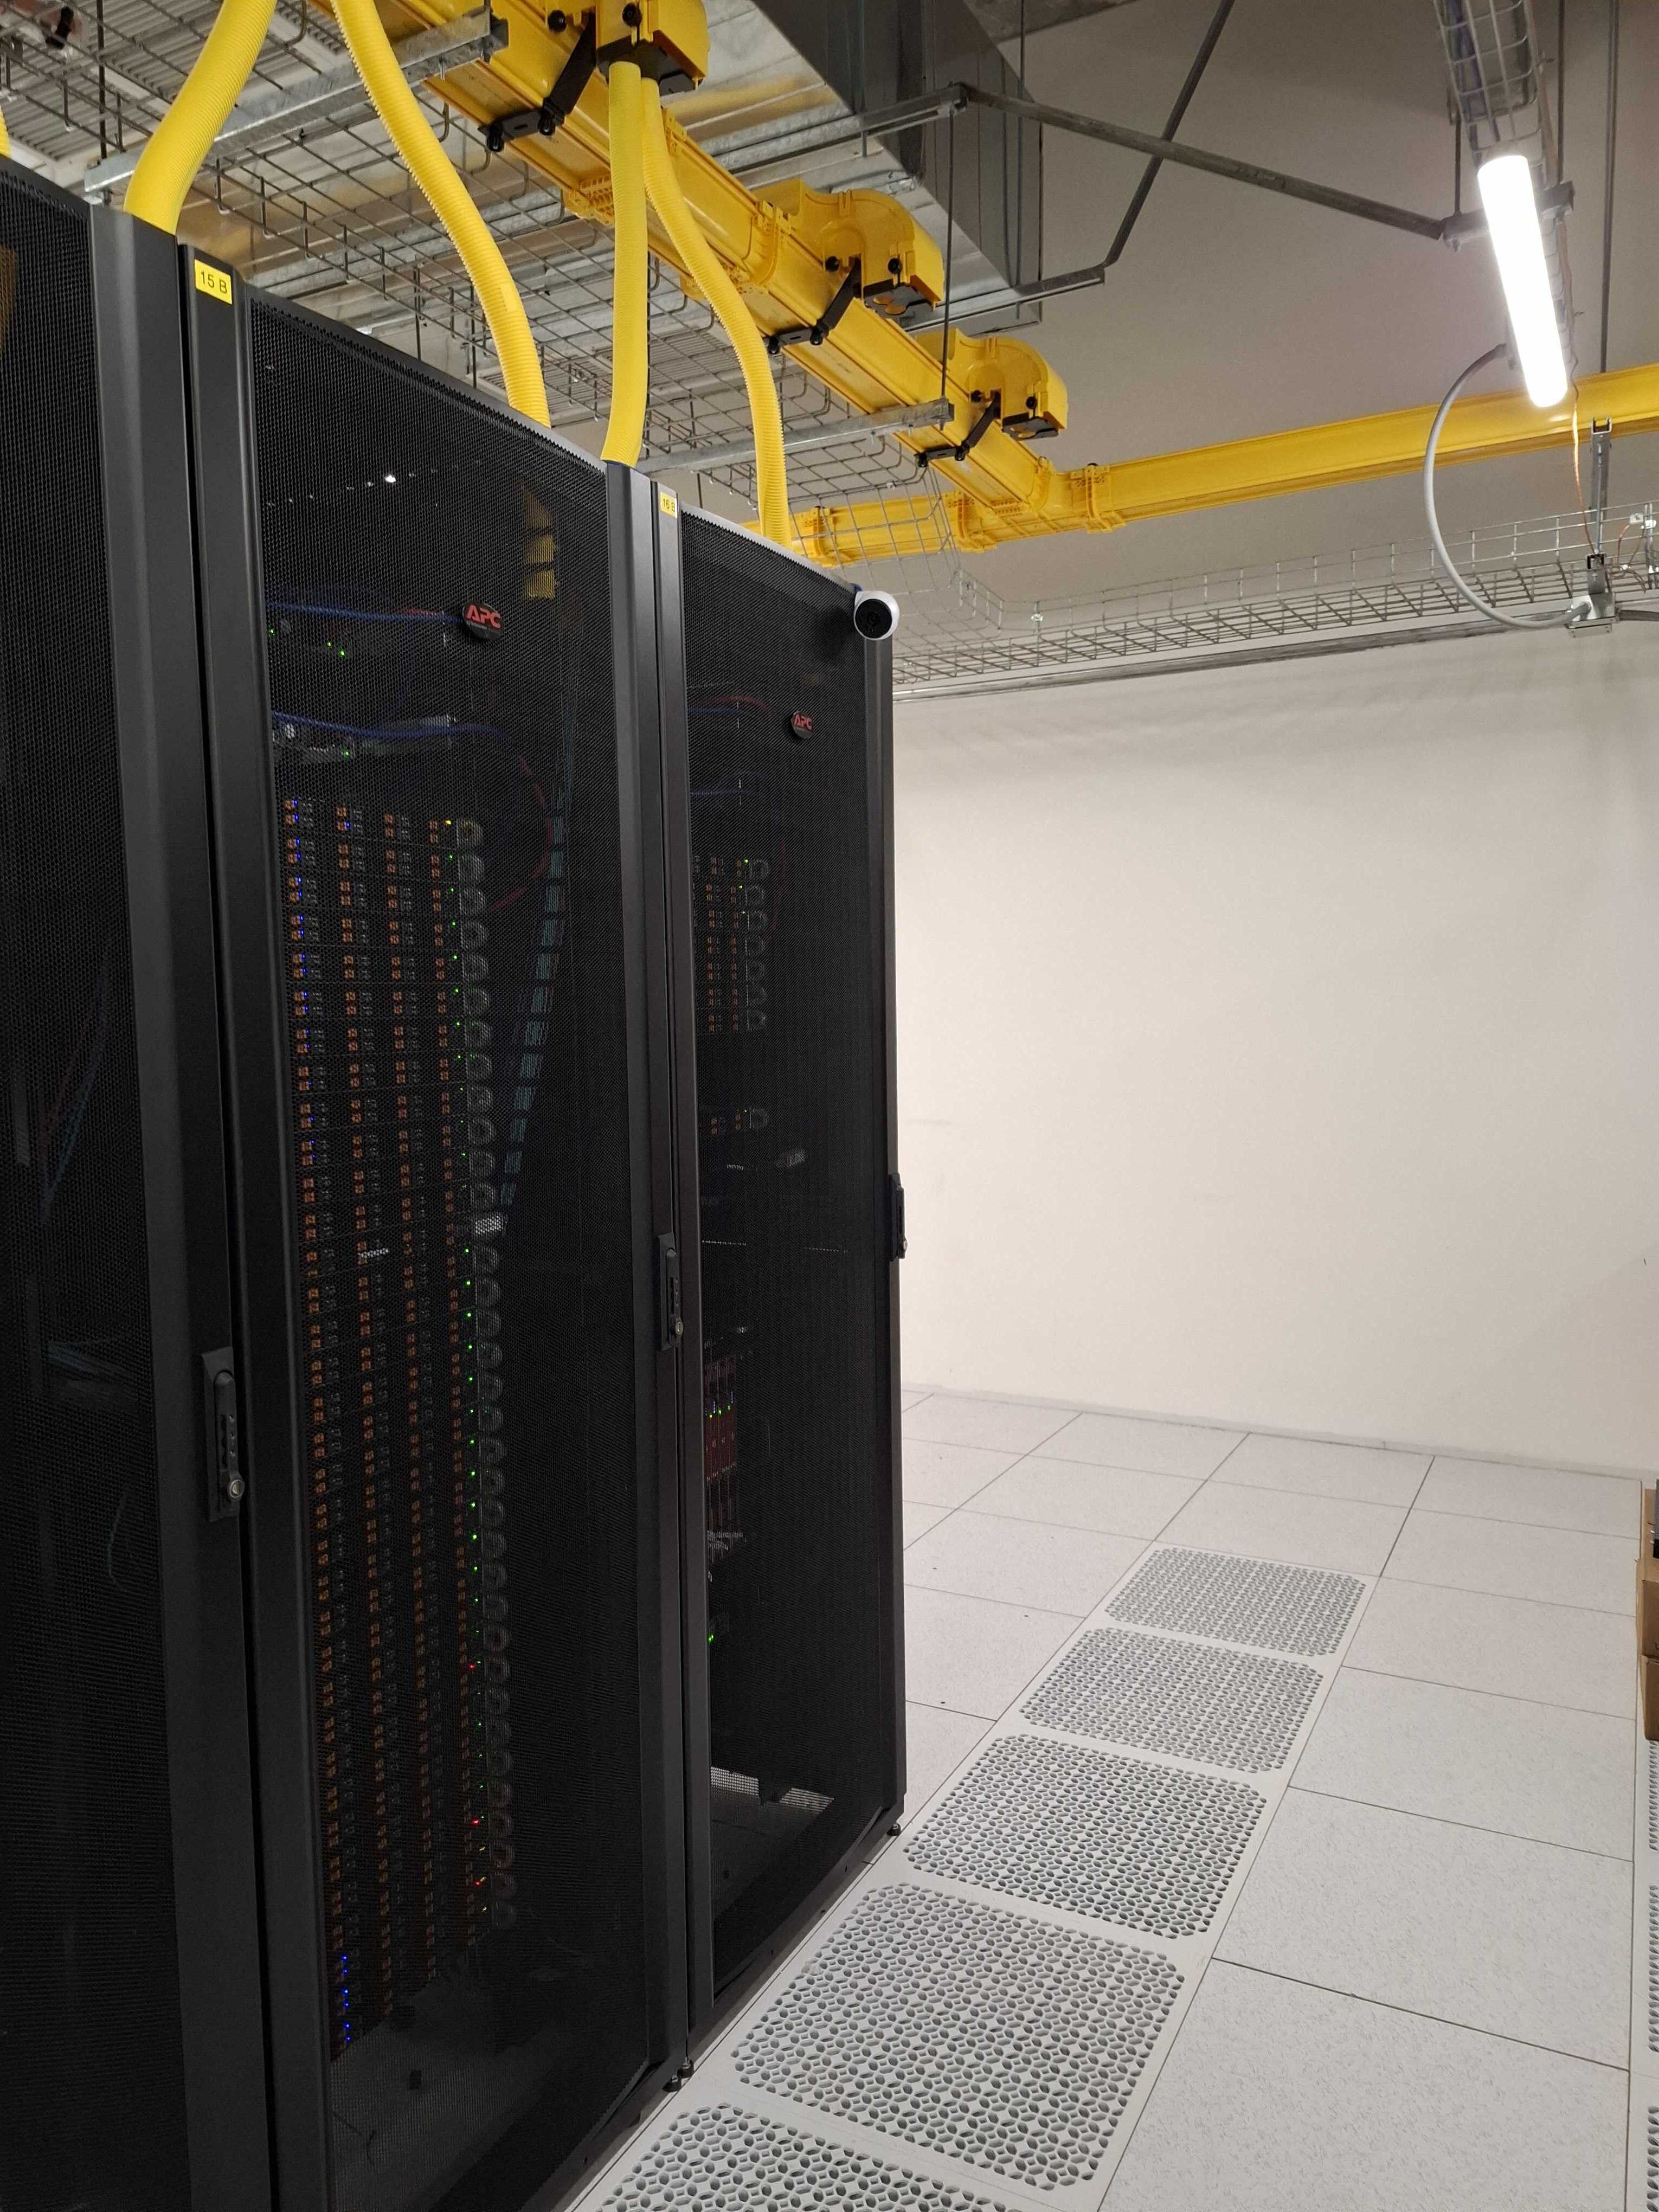
\includegraphics[width=8cm]{9.jpg}
    \centering
    \caption*{Cold Corridor Camera}
  \end{figure}

\subsection{Datacenter Cerro Pachon}

Here we have cameras pointing the first entrance called preparation room and we have cameras pointing front aisle of both rows and cameras pointing the back of both rows.

\begin{figure}
    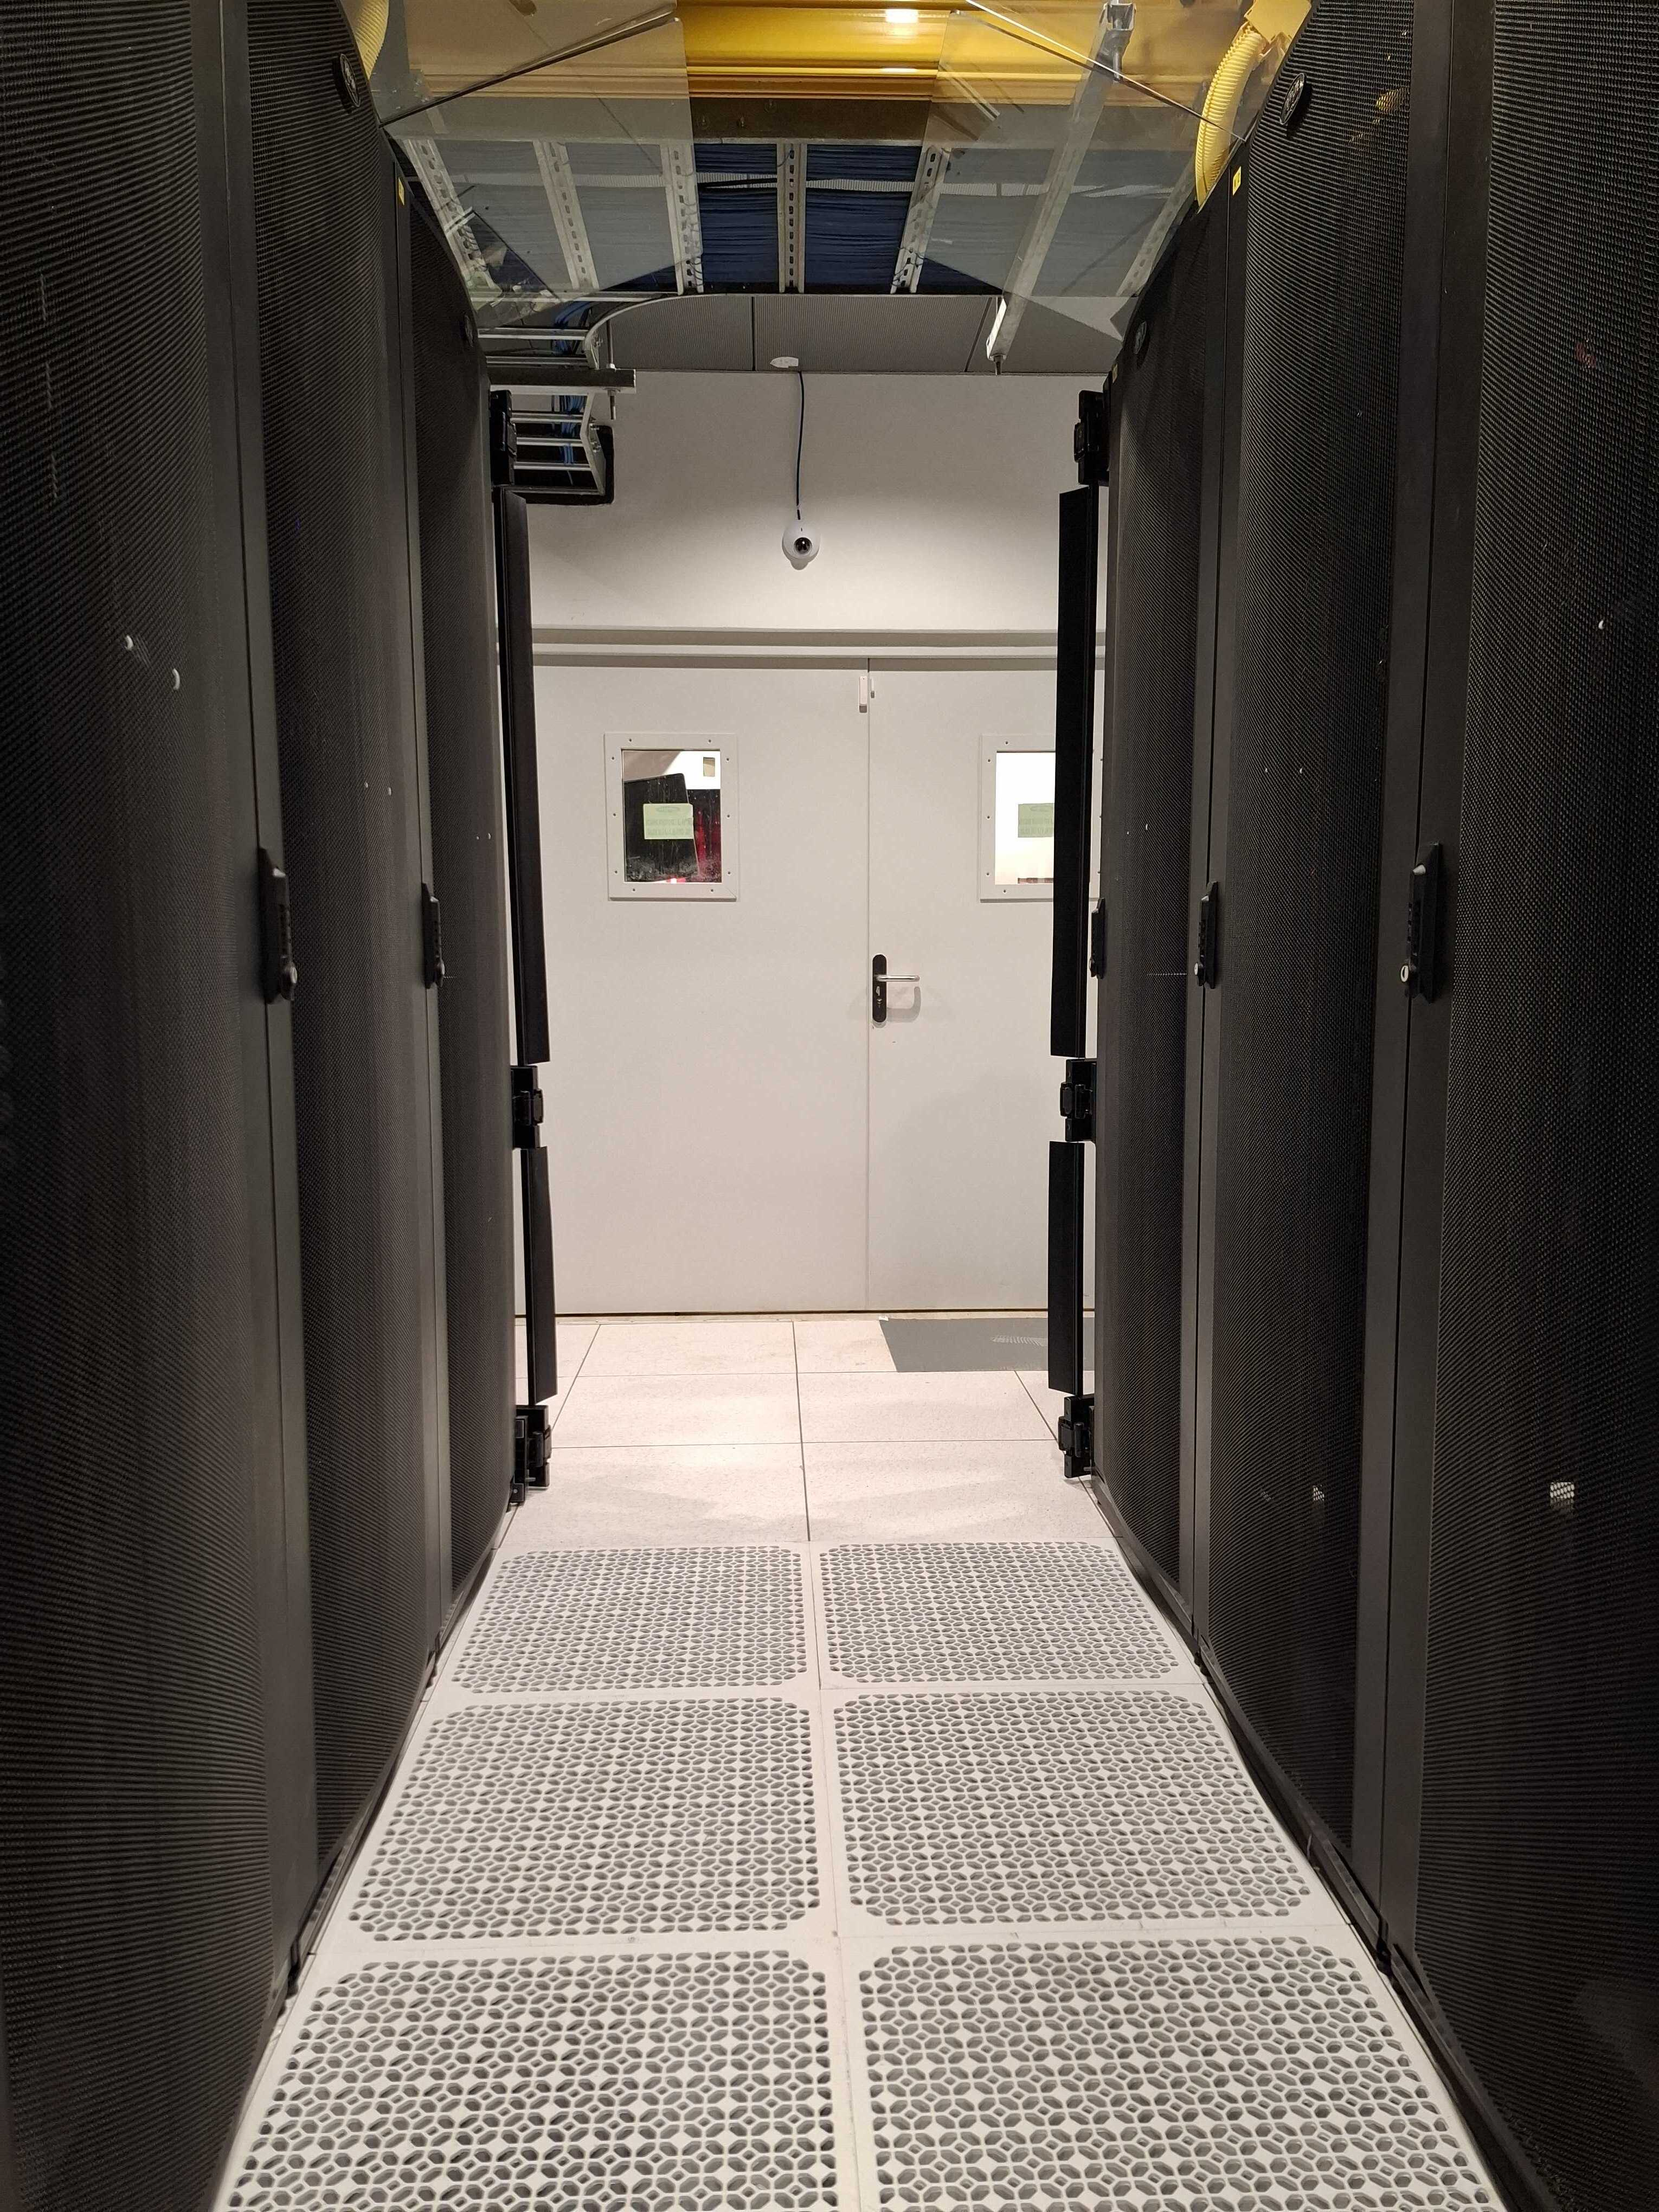
\includegraphics[width=6cm]{10.jpg}
    \centering
    \caption*{Cold Corridor Camera}
  \end{figure}
  \begin{figure}
    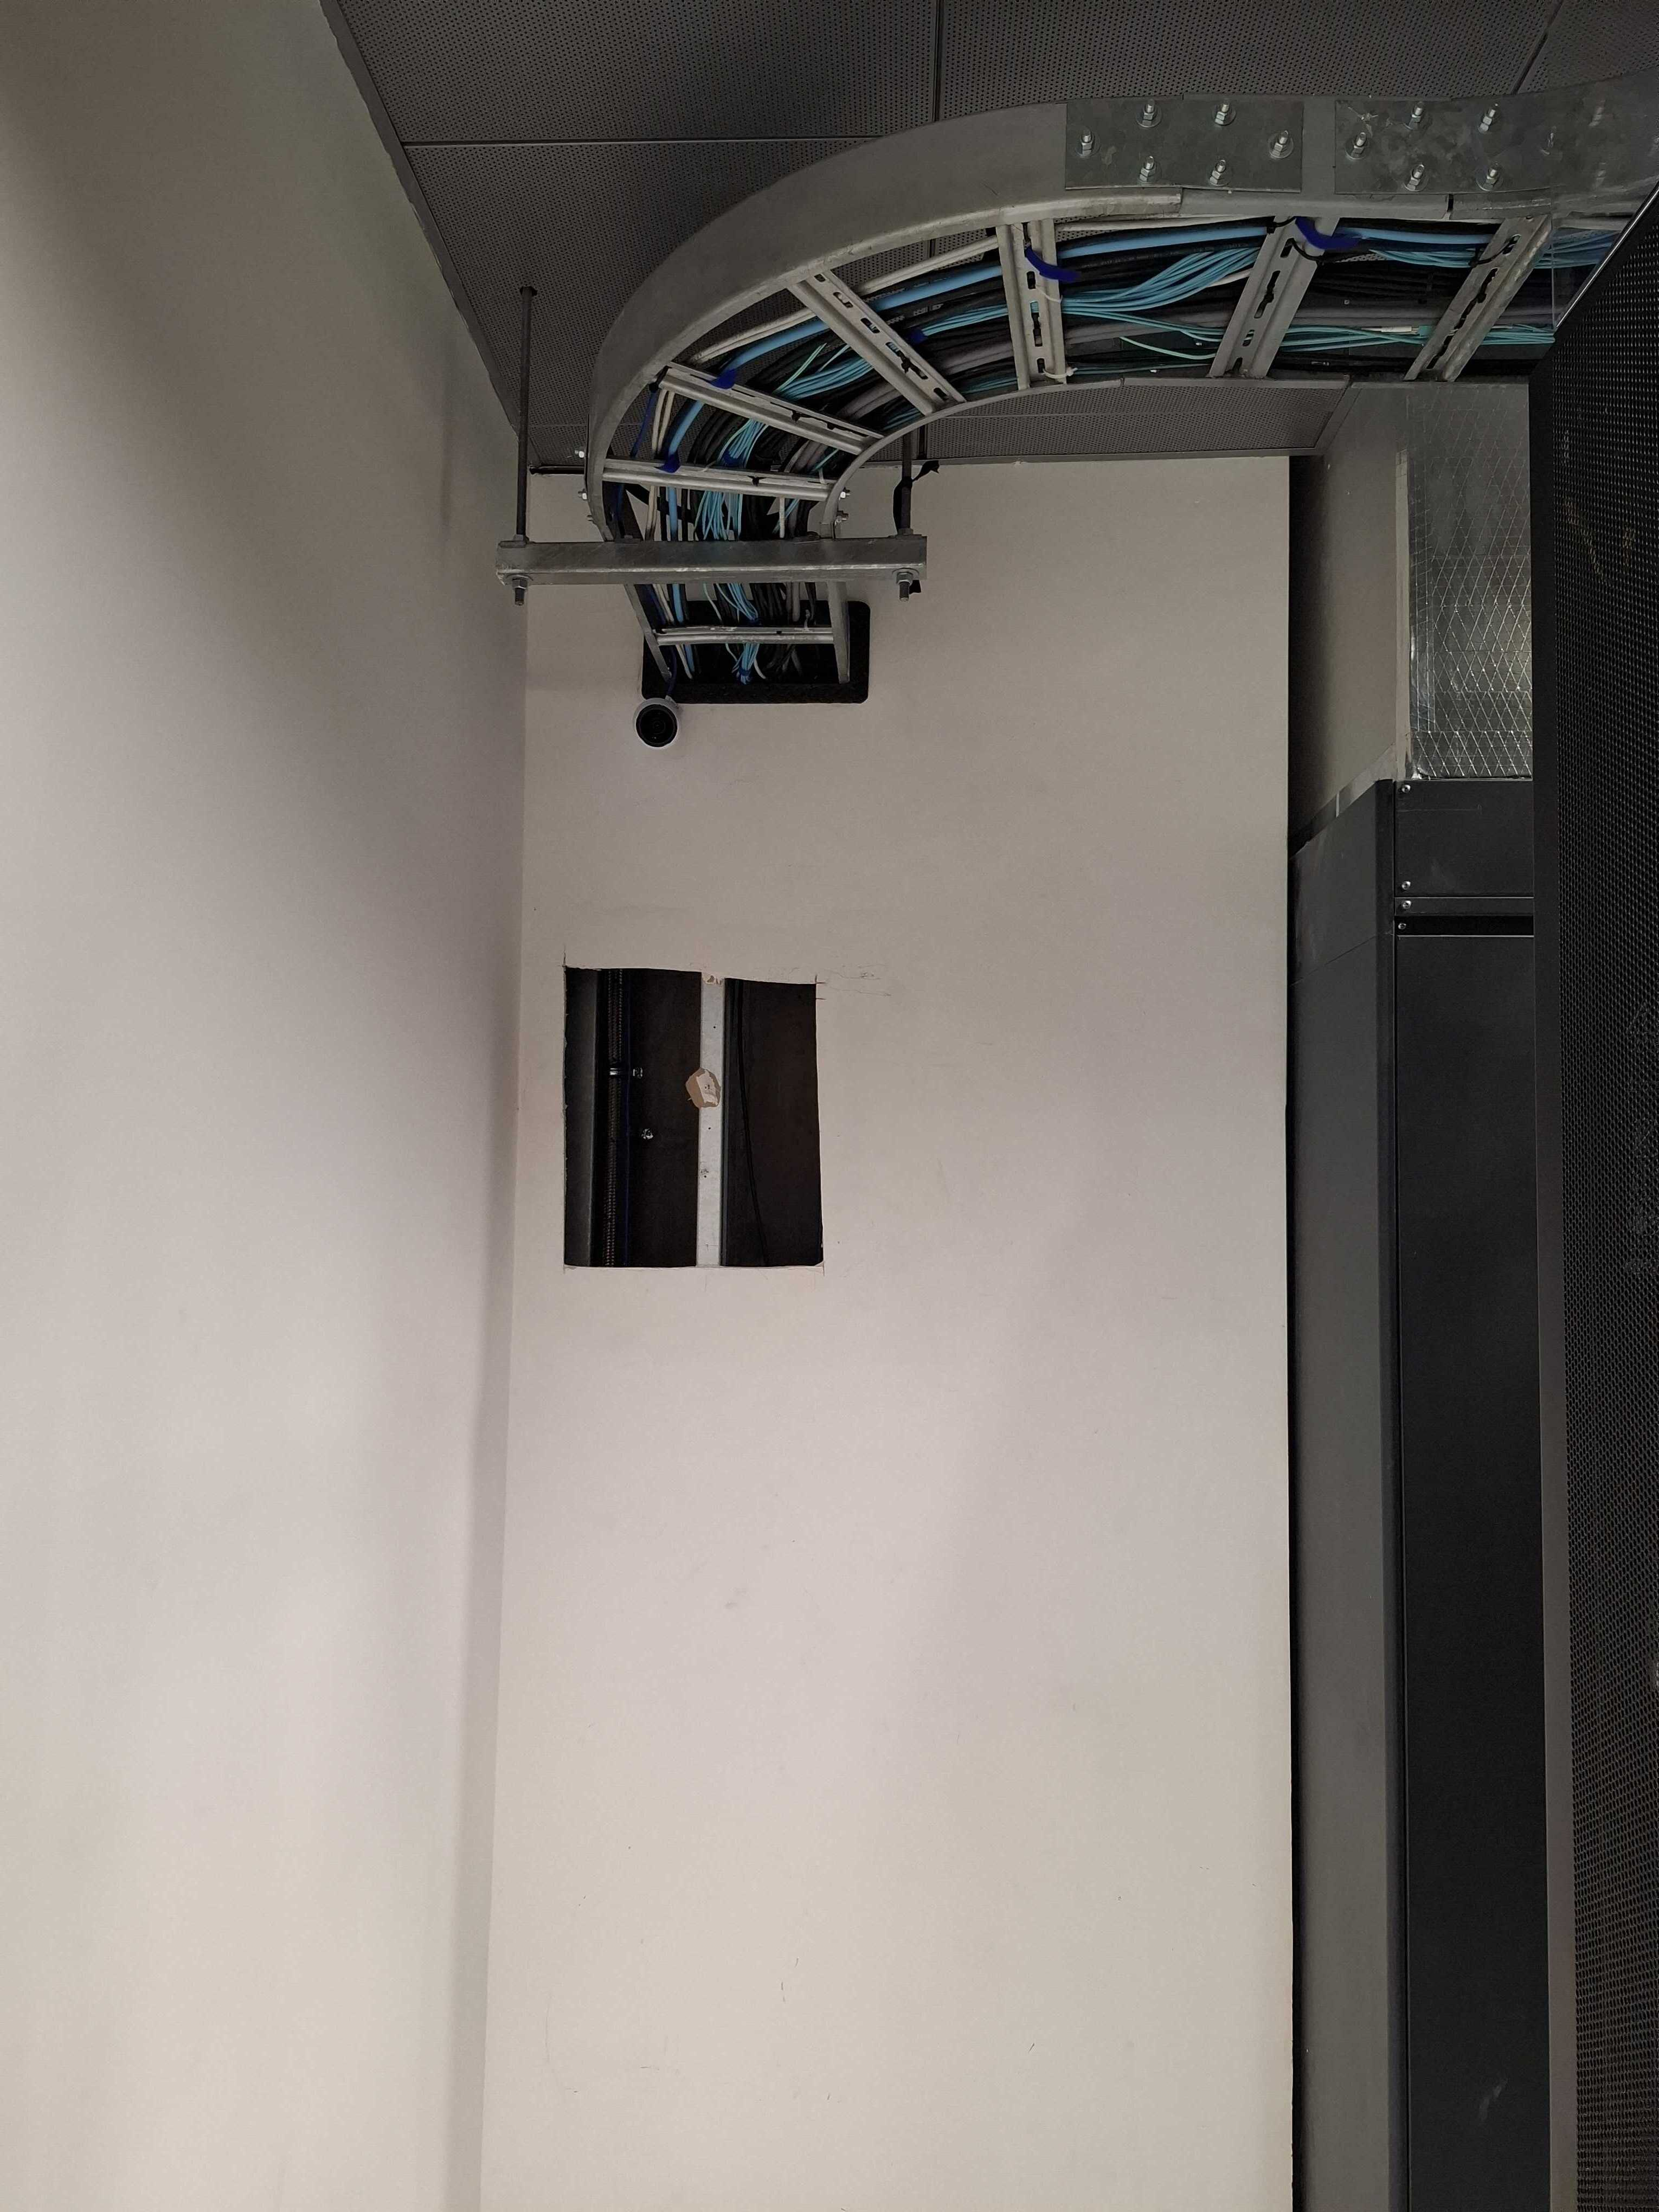
\includegraphics[width=6cm]{11.jpg}
    \centering
    \caption*{Hot Corridor Camera 1}
  \end{figure}
  \begin{figure}
    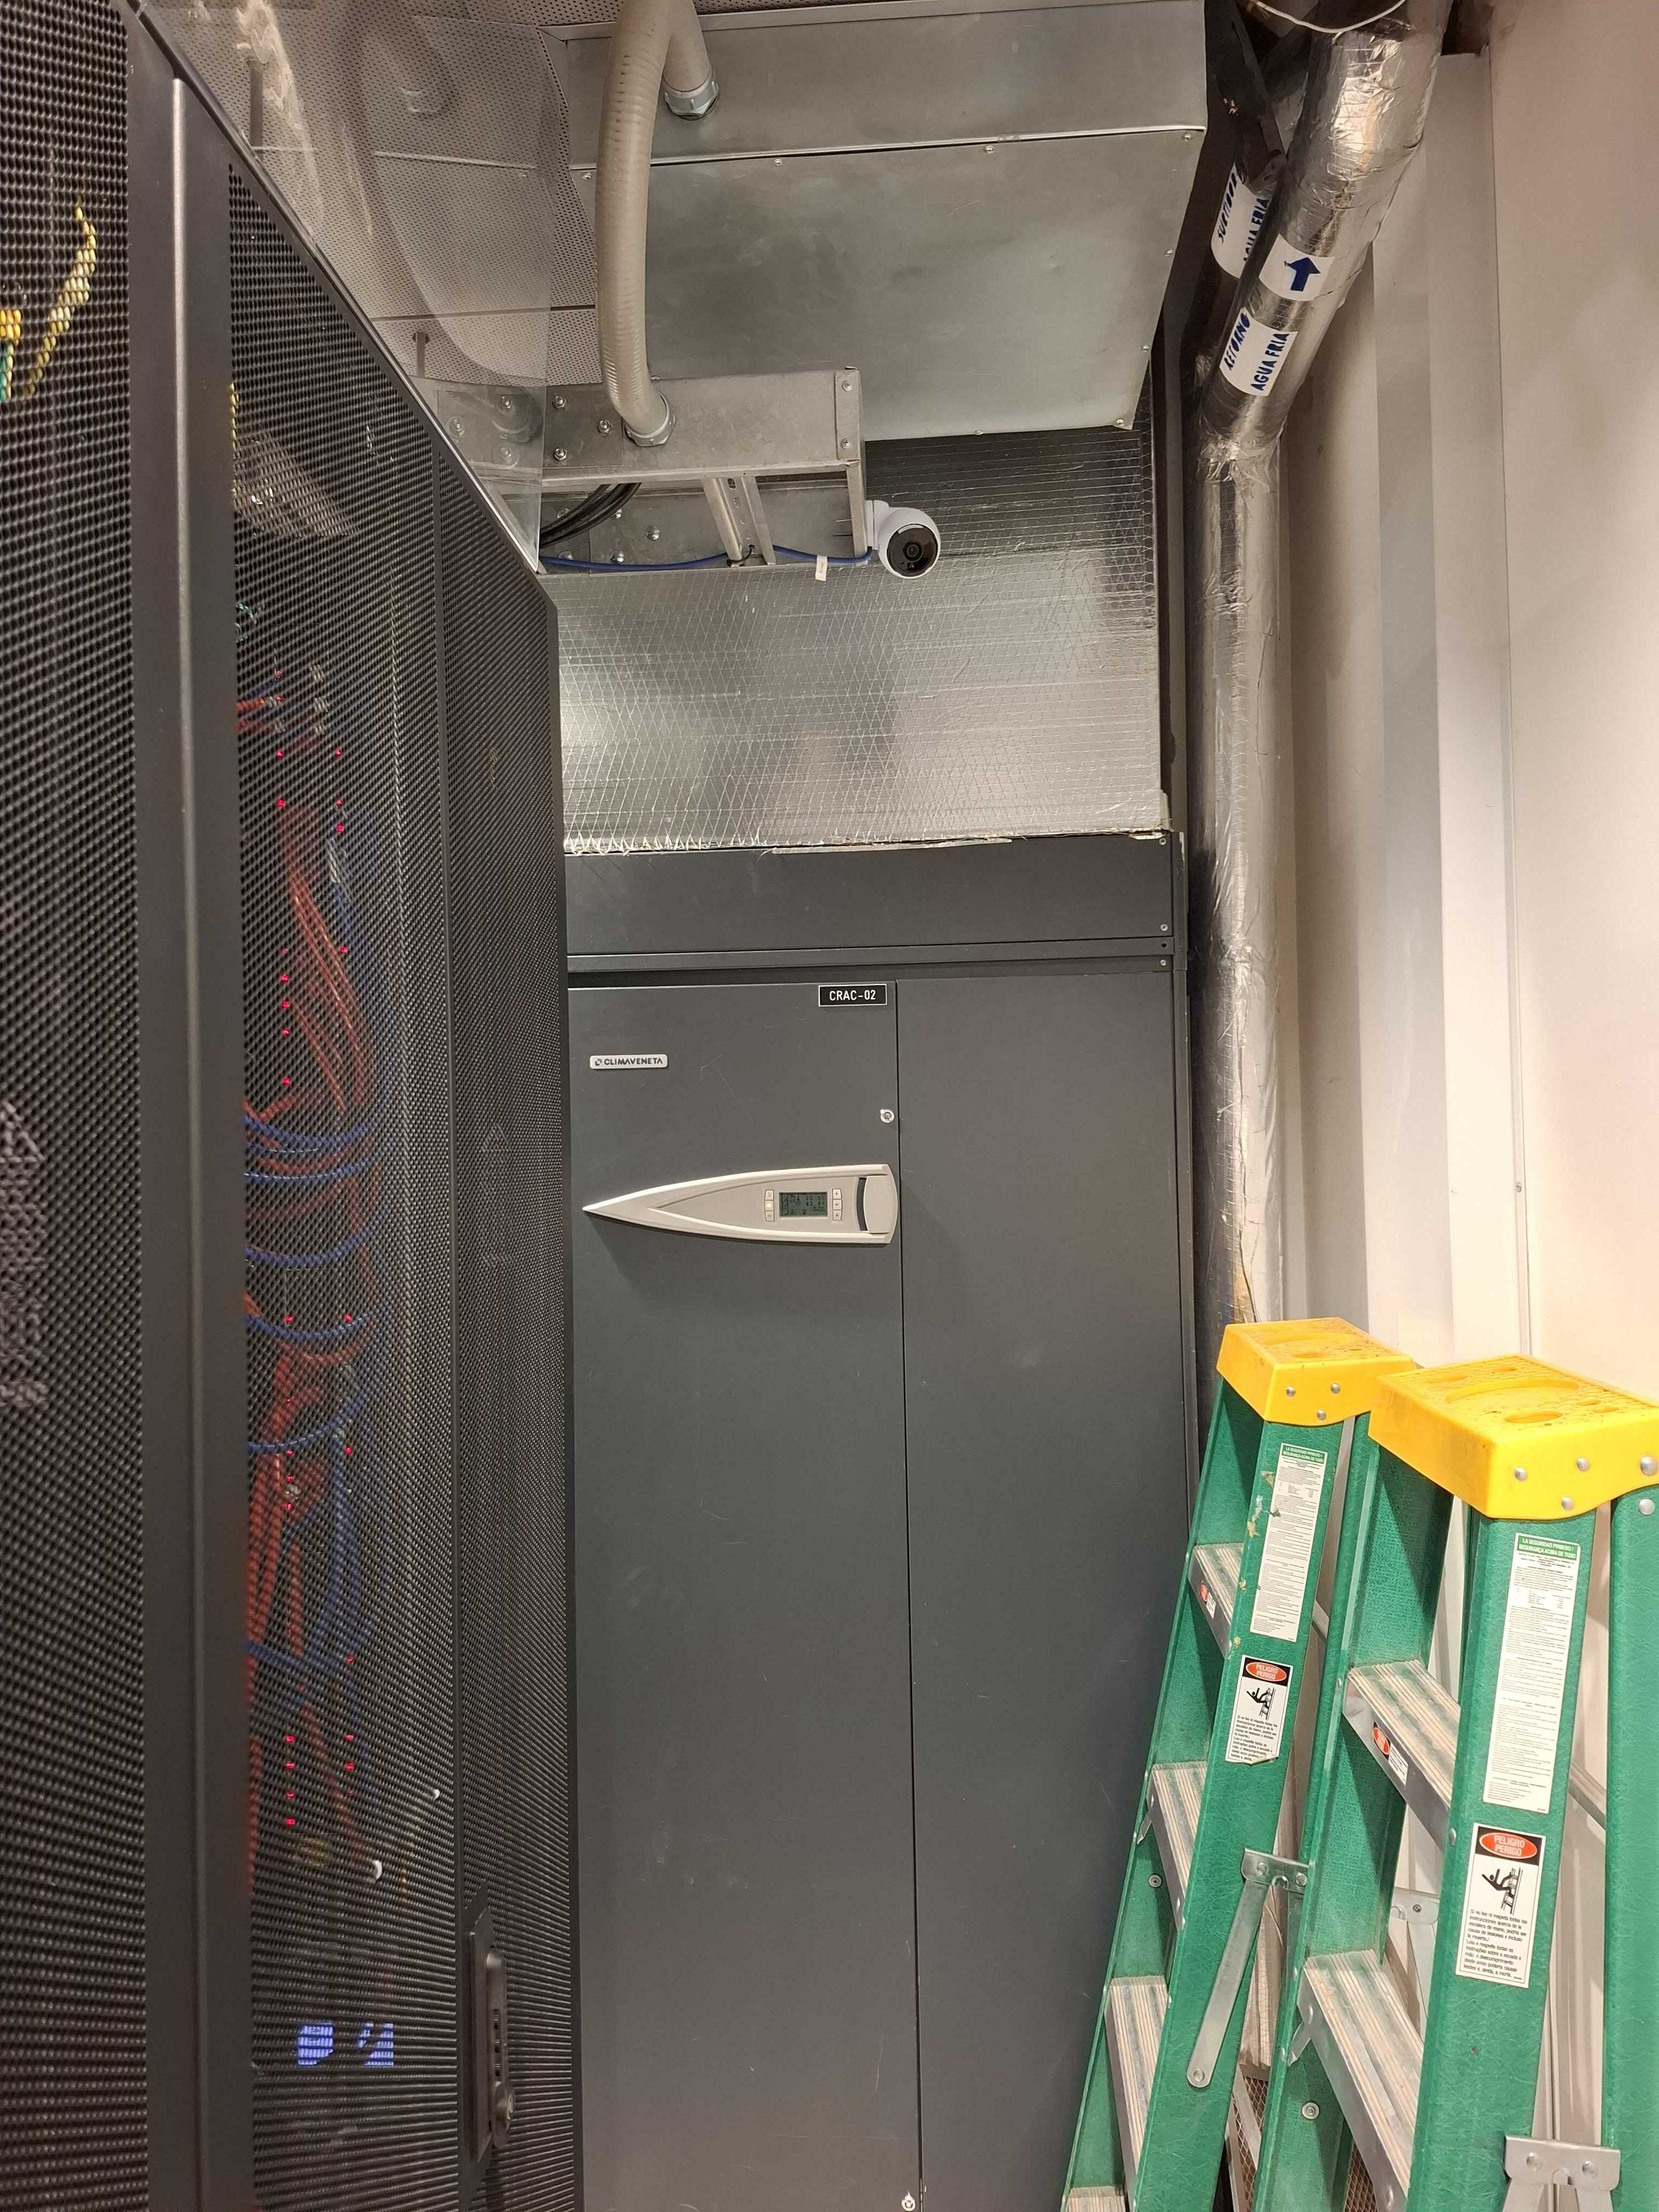
\includegraphics[width=6cm]{22.jpg}
    \centering
    \caption*{Hot Corridor Camera 2}
  \end{figure}

  \newpage

\section{Rack access control with open/close sensor system and security lock.}

The racks in both the data center in La Serena and the one in Cerro Pachón (Rubin) were fitted with magnetic sensors on the front and rear doors. These sensors are connected to a centralized system incorporated in each PDU of each rack independently of each other. These sensors announce door openings by leaving a time log and also at the time of closing this alarm is turned off. These announcements are visible both to the GUI of each PDU as a peripheral and also in a monitoring system.

\begin{figure}
    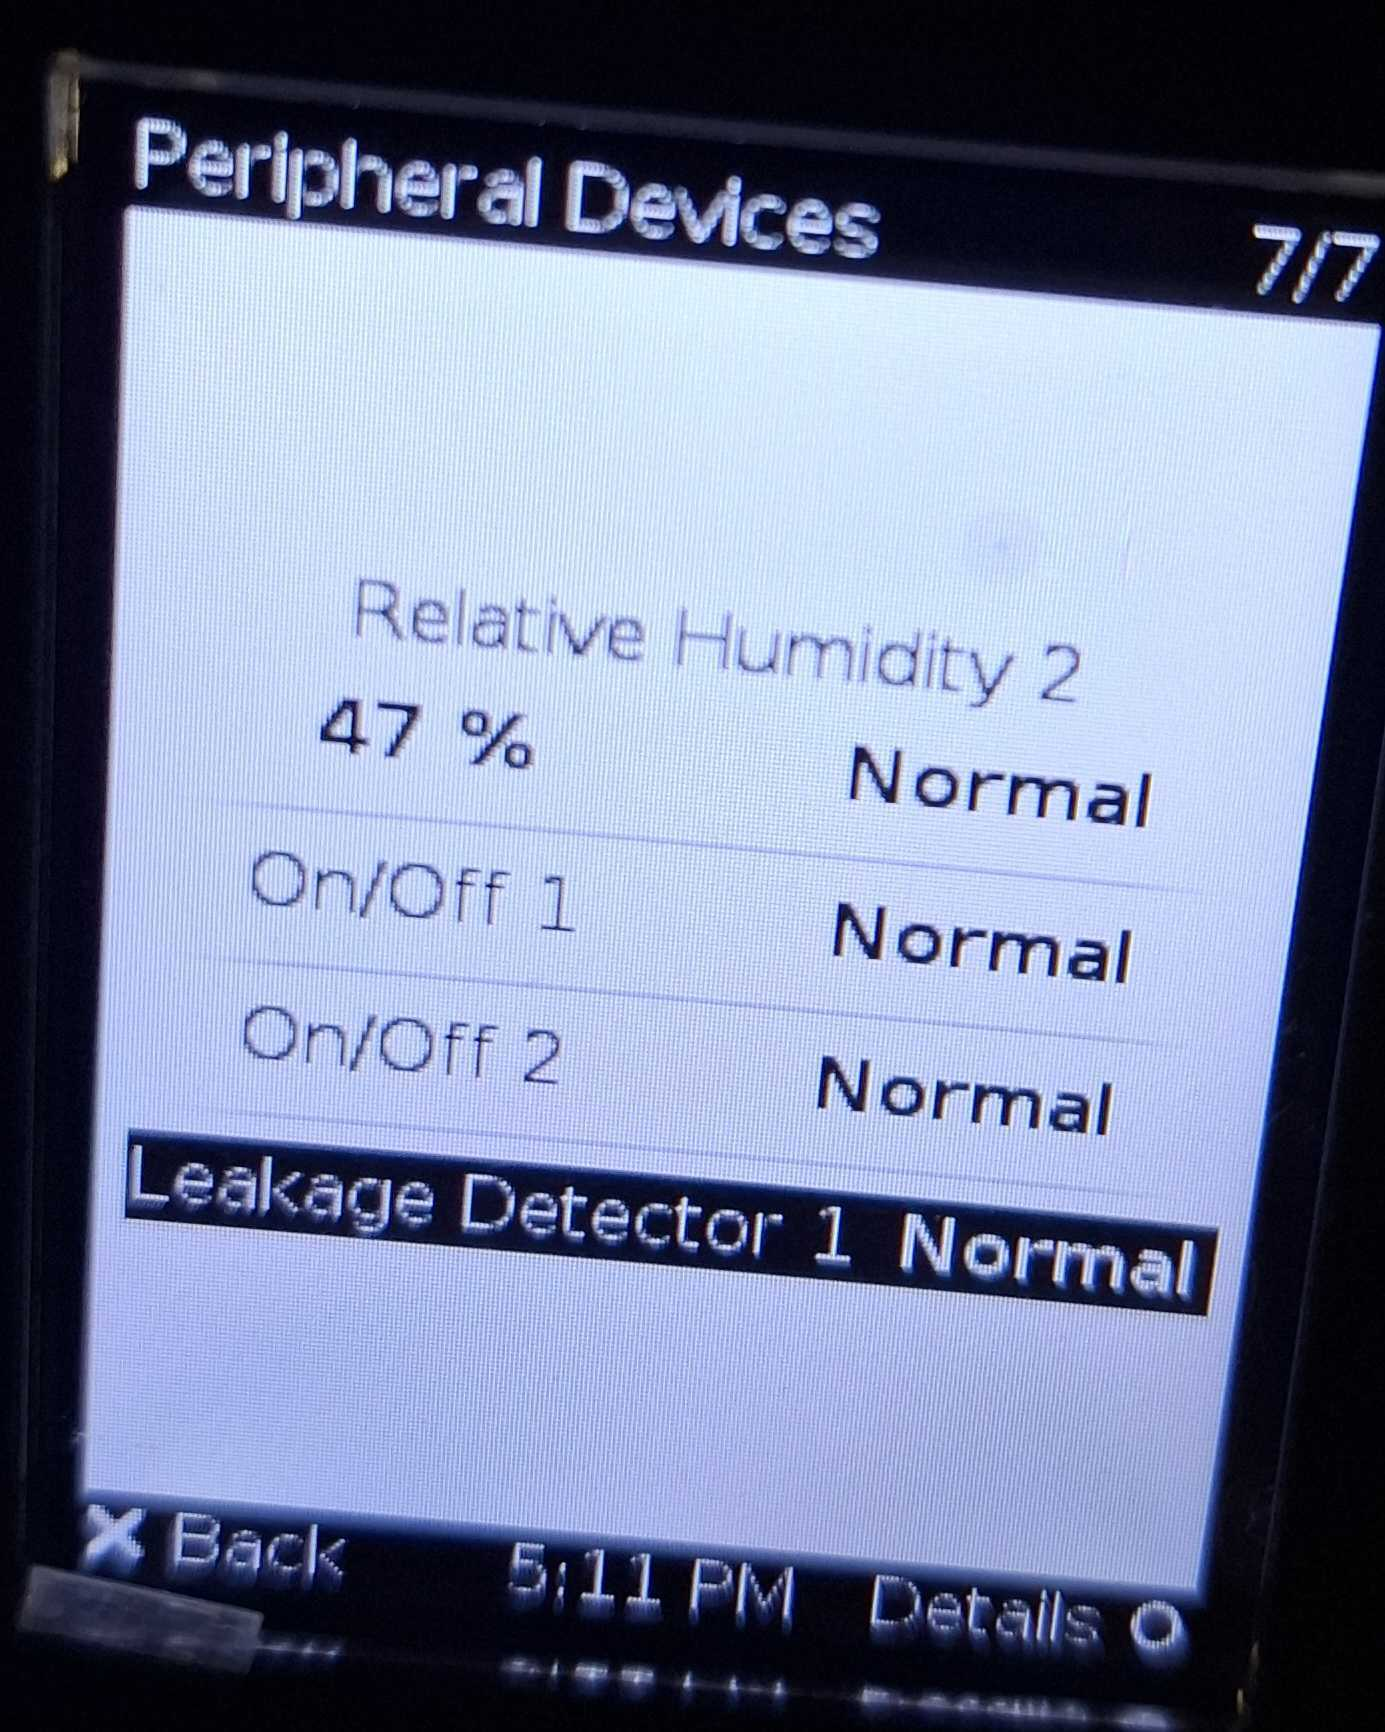
\includegraphics[width=5cm]{24.jpg}
    \centering
    \caption*{Sensor With Open Doors}
  \end{figure}
  \begin{figure}
    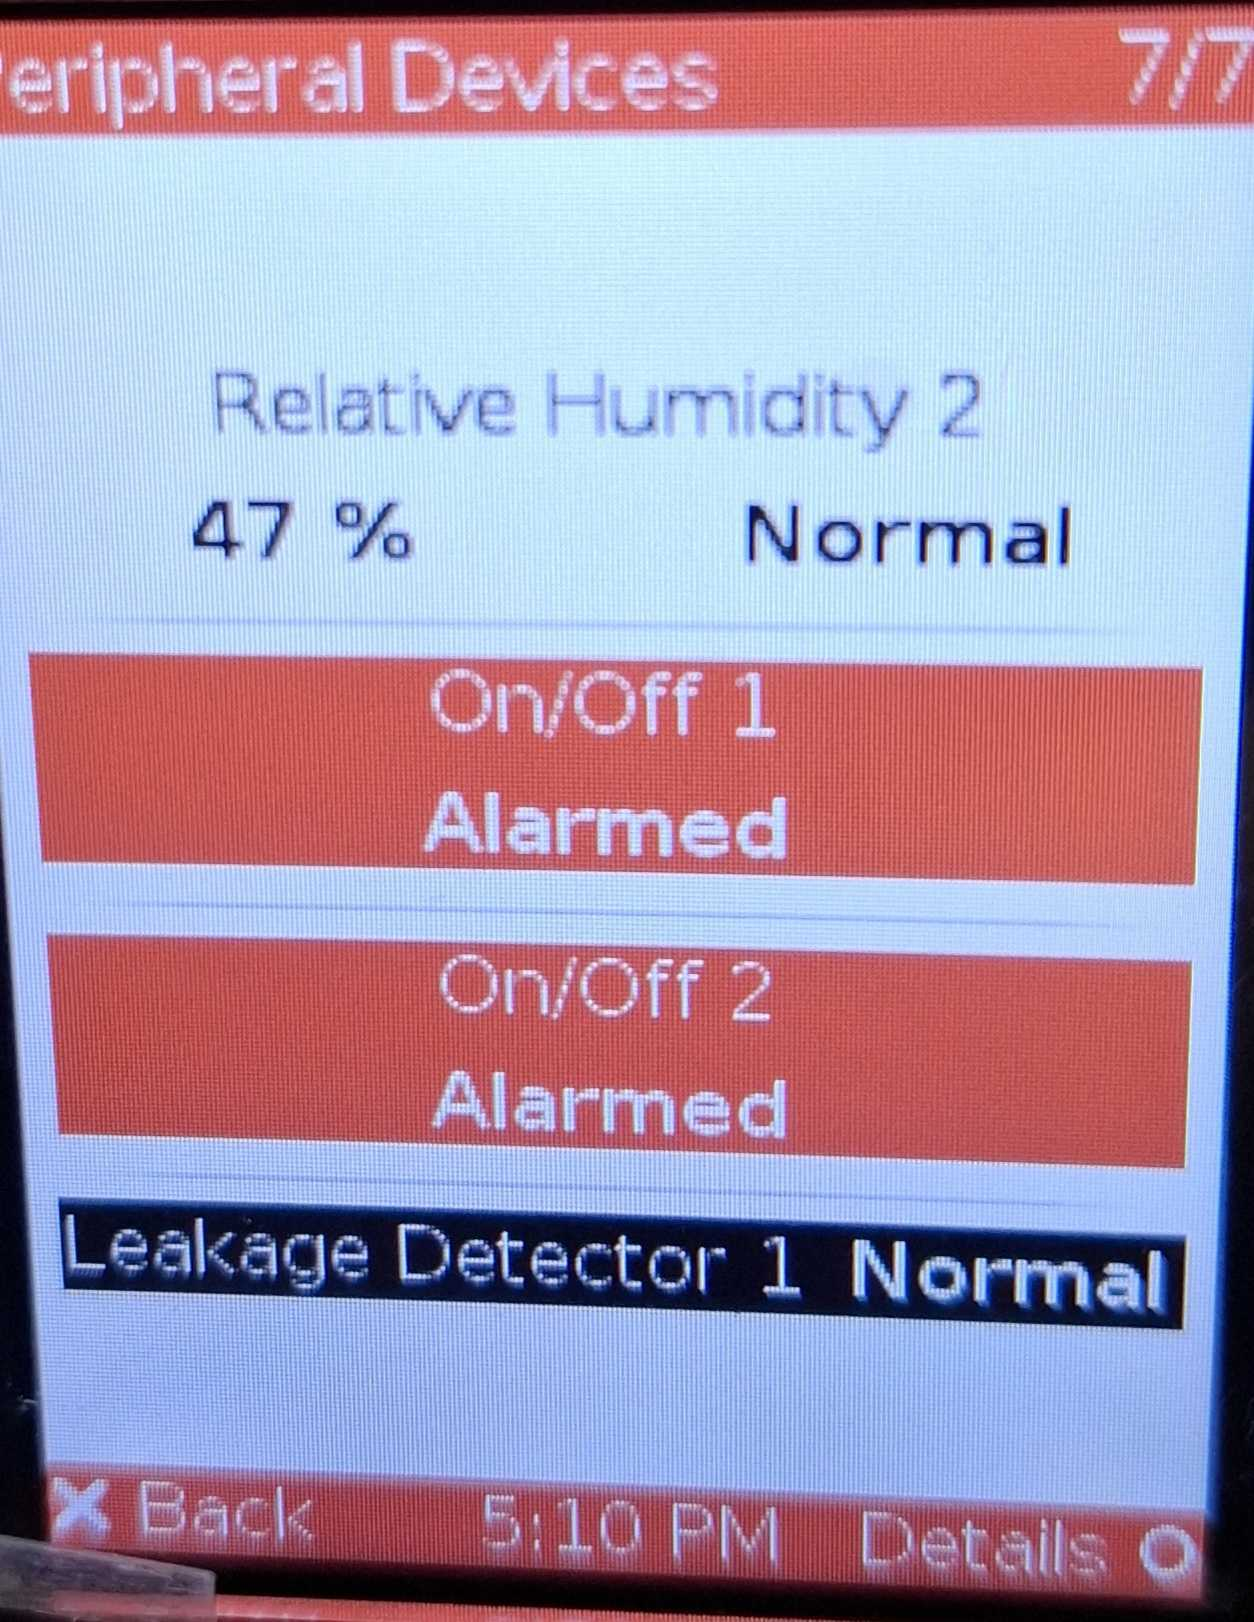
\includegraphics[width=5cm]{23.jpg}
    \centering
    \caption*{Sensor With Closed Doors}
  \end{figure}
  \begin{figure}
    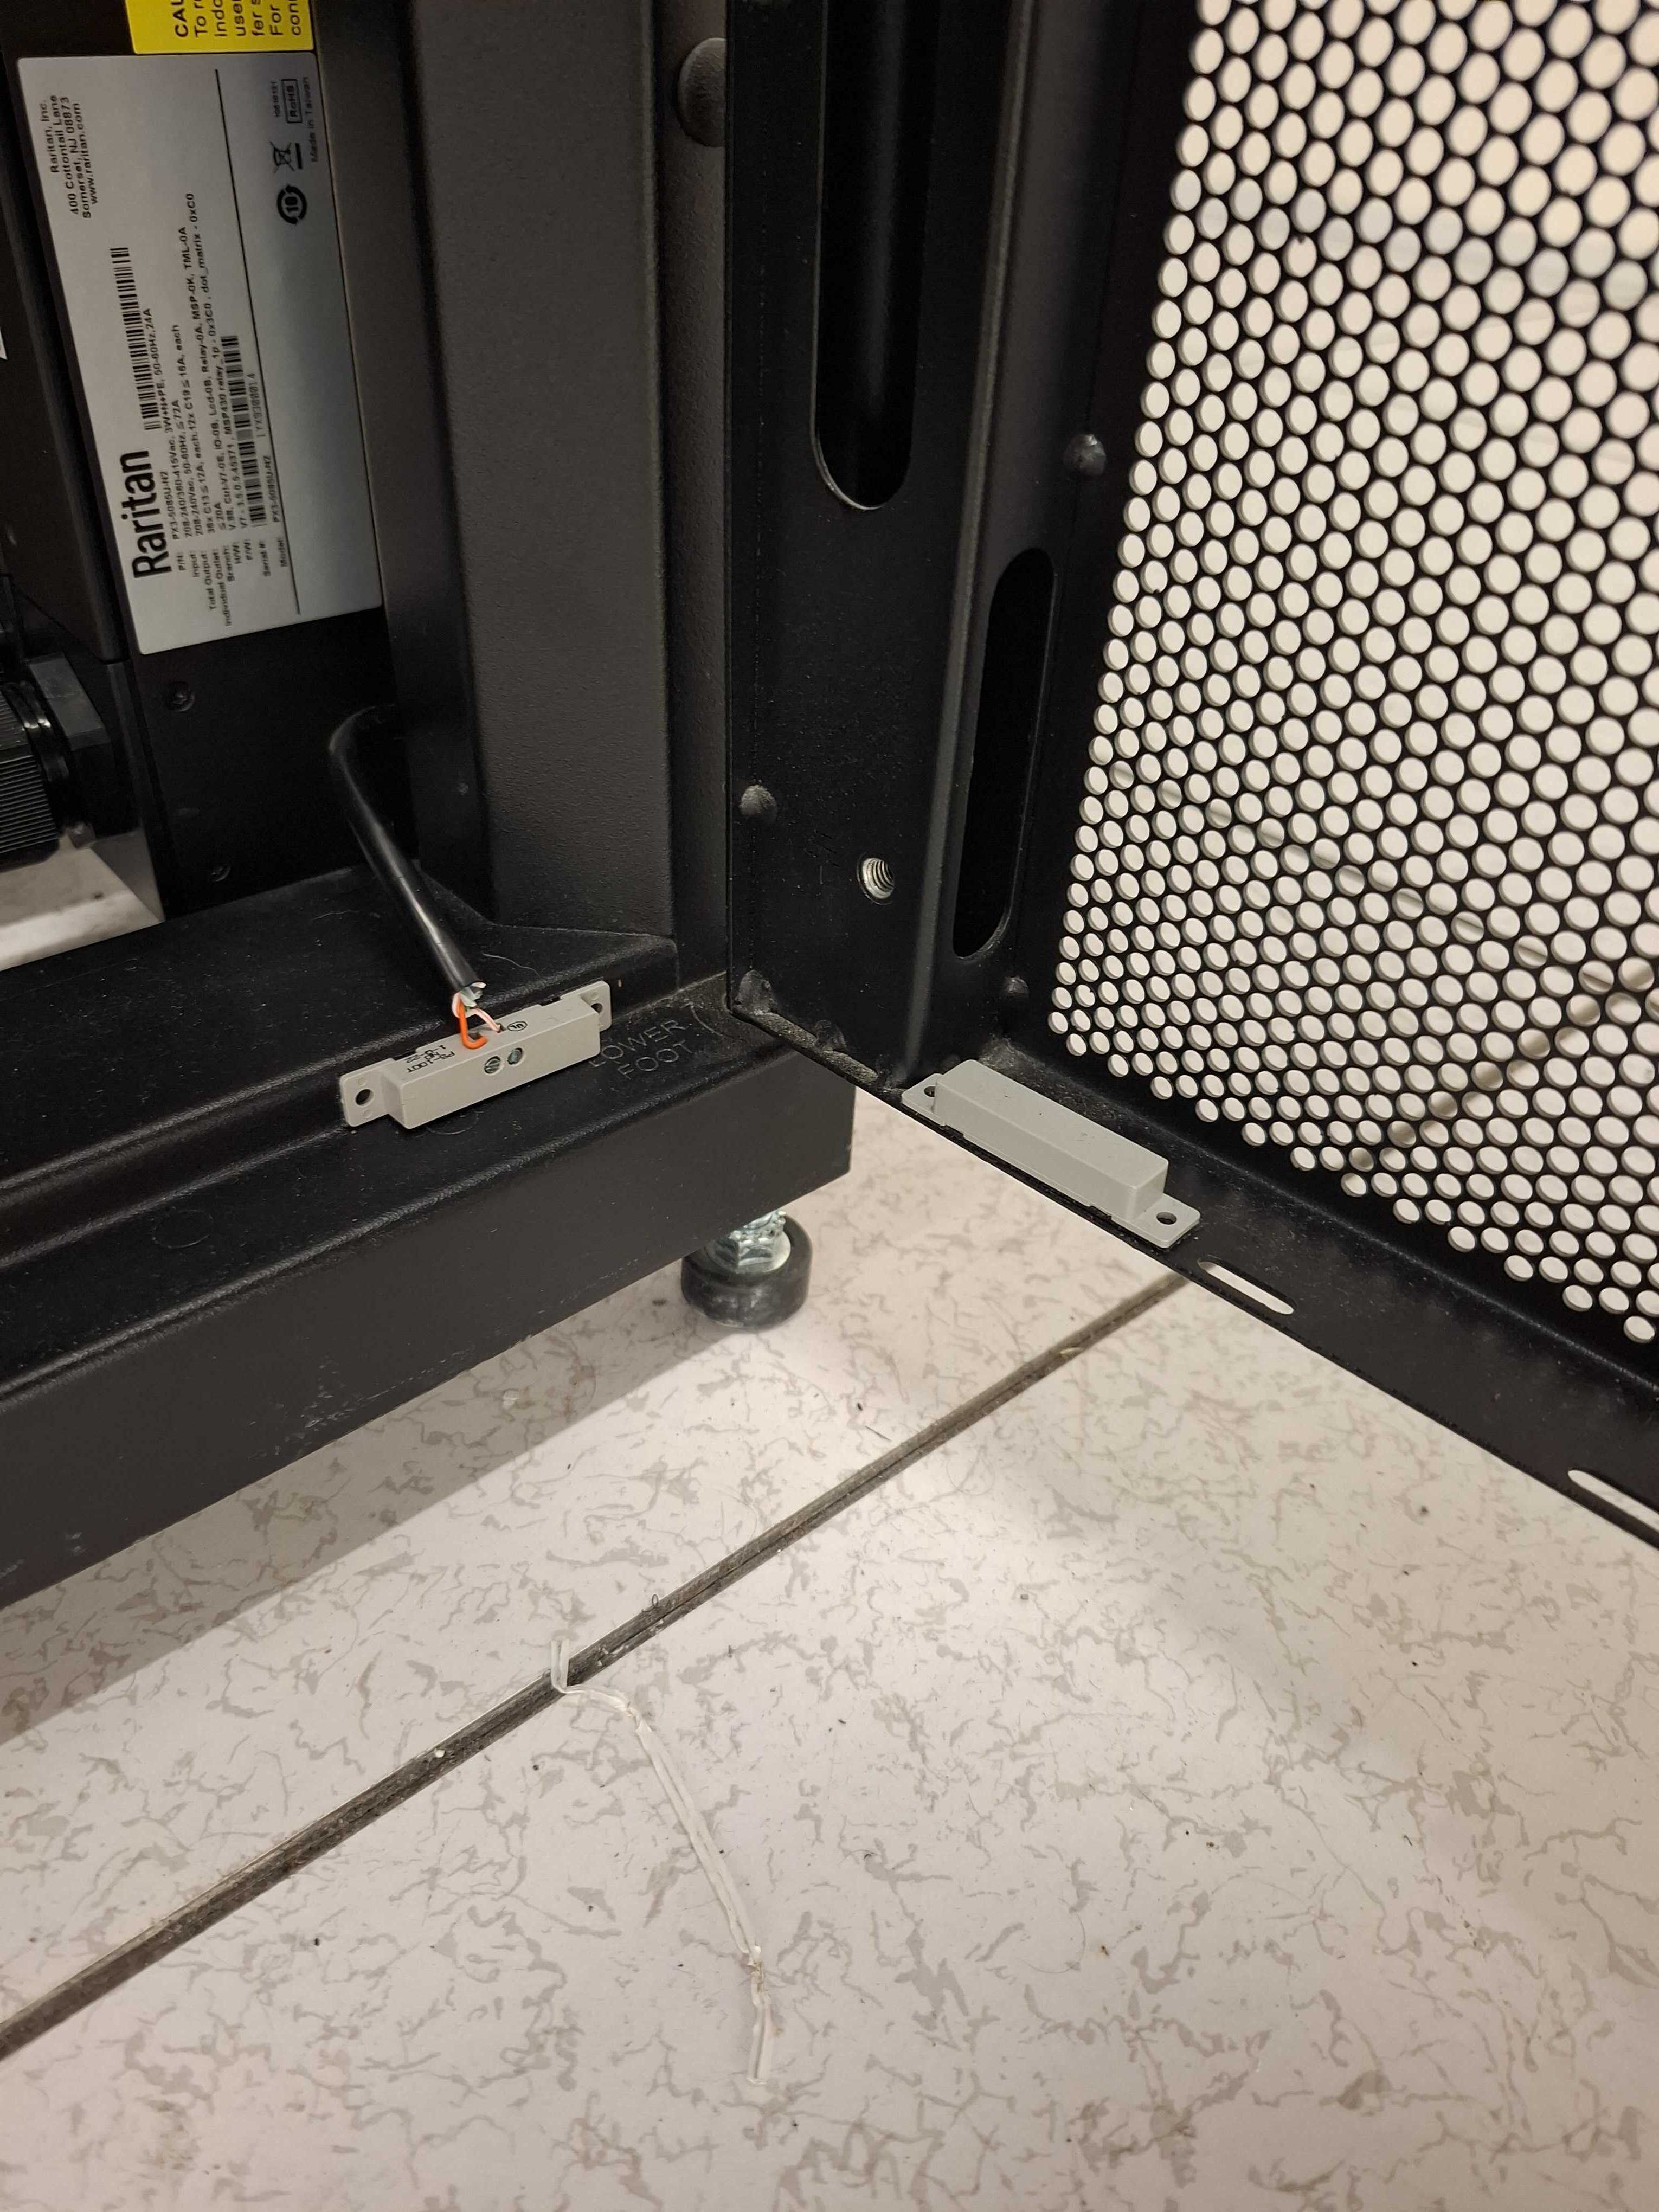
\includegraphics[width=5cm]{25.jpg}
    \centering
    \caption*{Magnetic Sensor}
  \end{figure}

  \newpage

The racks are also access controlled with Combination Lock on all racks on both front and rear doors. The combination is held by IT team.

\begin{figure}
    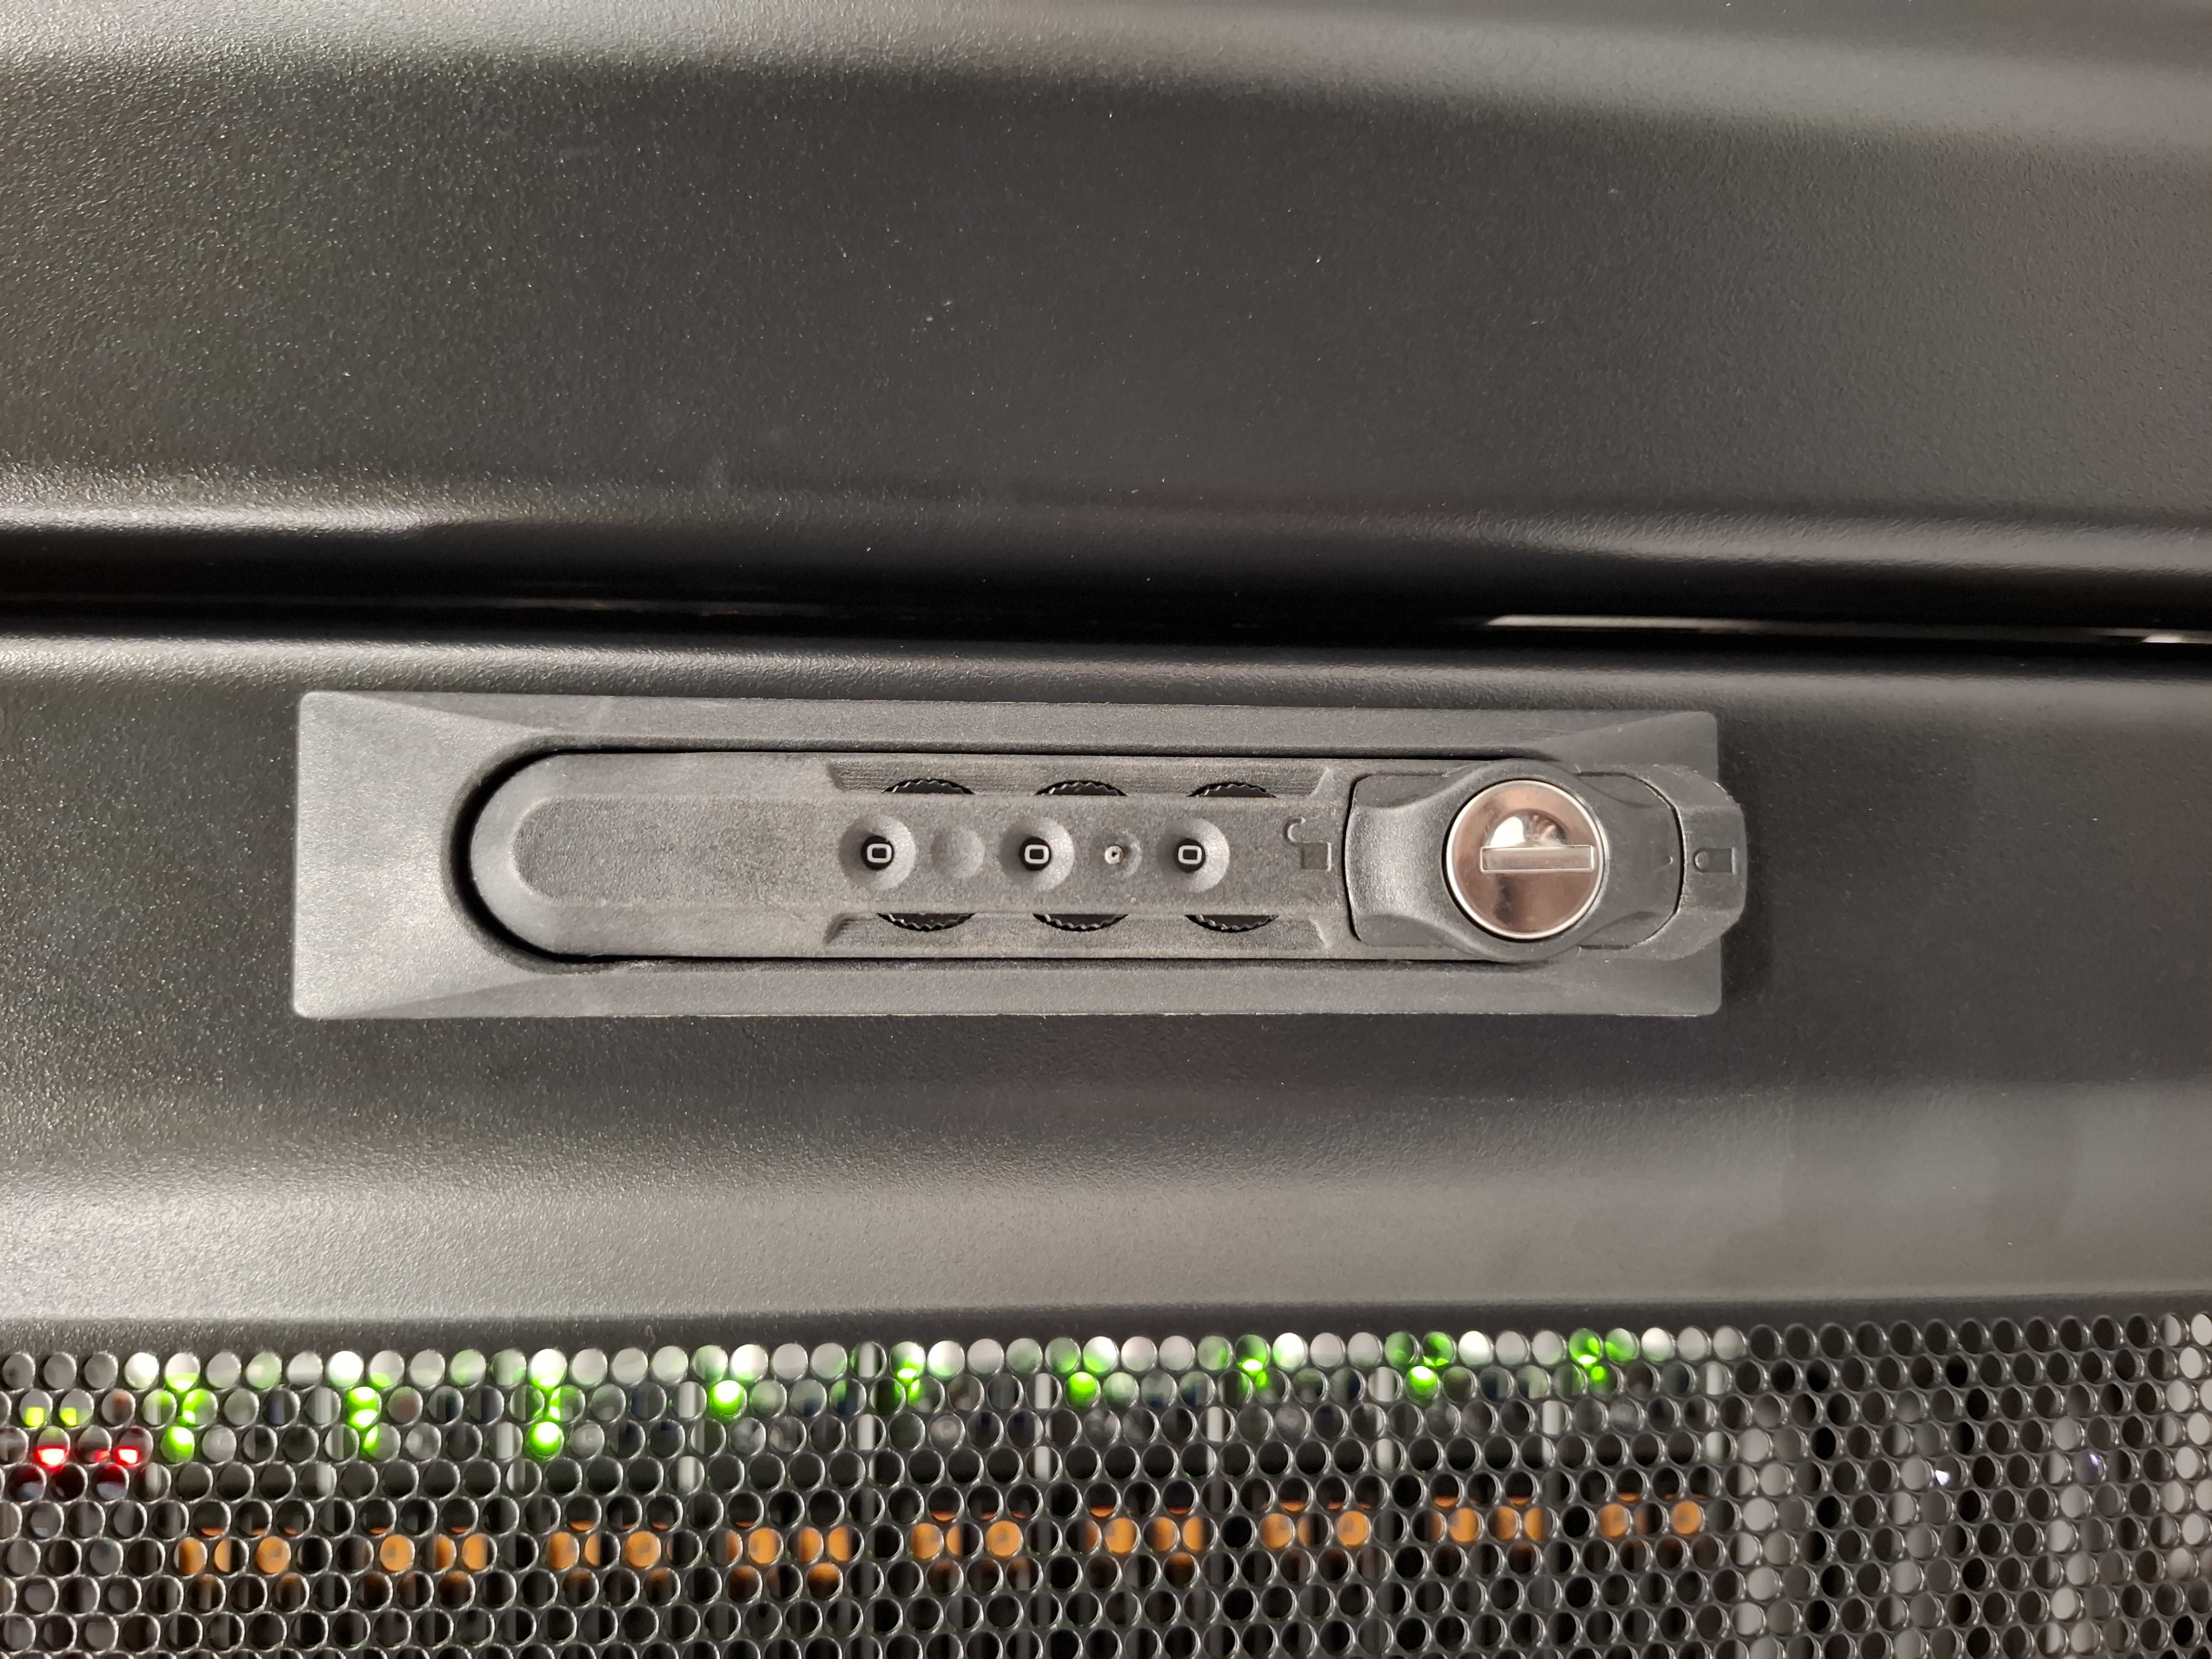
\includegraphics[width=10cm]{27.jpg}
    \centering
    \caption*{Combination Lock}
  \end{figure}

  \newpage
